\begin{bt}%[1D7H1-5]
% nguon: Archive/SP_SauLuoi_2024-2025/SP_GHKI/2-TN-DS-TLN-THPT-NgoGiaTu-DakLak-GHKI-NH24-25.tex #124
%[Dự án đề kiểm tra Toán khối 12 GHKI NH24-25 Đợt 2-Hieu Hieu Minh Minh]%[THPT NgoGiaTu-DakLak]
	Giả sử số dân của một thị trấn sau $t$ năm kể từ năm $1970$ được mô tả bởi hàm số $f(t)=\dfrac{26 t+10}{t+5}$, $t \geq 0$, trong đó $f(t)$ được tính bằng nghìn người. Đạo hàm của hàm số $f(t)$ biểu thị tốc độ tăng dân số của thị trấn đó (tính bằng nghìn người/năm). Tính tốc độ tăng dân số của thị trấn đó vào năm $1985$ (kết quả tính bằng nghìn người/năm).
	\shortans[oly]{0,3}
	\loigiai{
		Ta có $t=1985-1970=15$ và $f'(t)=\dfrac{120}{(t+5)^2}$.\\	
		Tốc độ tăng số dân vào năm $1985$ là $f'(15)=\dfrac{120}{(15+5)^2}=\dfrac{120}{20^2} = 0{,}3$ nghìn người/năm.
	}
\end{bt}

\begin{bt}%[1D7H2-2]
% nguon: Archive/2024/TOAN_11_XE/TOAN_11_XE/data4/11C9/BTTN2.tex #1317
%[Thy Nguyen Vo Diem]%
	Cho hai hàm số $y_1=\sin^4x+\cos ^4x$ và $y_2=\dfrac{1}{4}\cos 4x$. Chứng minh $y_1'=y_2'$.
	\loigiai{
		$y_1=(\sin^2x+\cos^2x)^2-2\sin^2 x\cos^2 x=1-\dfrac{1}{2}\sin^2 2x$\\
		$\Rightarrow y_1'=-\dfrac{1}{2}\cdot 2\sin 2x \cdot 2\cos 2x=-\sin 4x$.\\
		$y_2=\dfrac{1}{4}\cos 4x \Rightarrow y_2'=-\dfrac{1}{4}\cdot 4 \sin 4x=-\sin 4x$.\\
		Vậy $y_1'=y_2'$.
	}
\end{bt}

\begin{ex}%[1D7V2-8]
% nguon: Archive/2024/TaiLieuGiangDay/1.HamSo/1. K12 - 4in1 - Hamso/ThubaiGoc/Bai5-Dang11.tex #2408
%[Tên dự án, Tên GV]%Sách CD-1-4-BT11
	Một tàu đổ bộ tiếp cận Mặt Trăng theo cách tiếp cận thẳng đứng và đốt cháy các tên lửa hãm ở độ cao $250$ km so với bề mặt của Mặt Trăng.\\
	Trong khoảng $50$ giây đầu tiên kể từ khi đốt cháy các tên lửa hãm, độ cao $h$ của con tàu so với bề mặt của Mặt Trăng được tính (gần đúng) bởi hàm $h(t)=-0{,}01t^3+1{,}1t^2-30t+250$, trong đó $t$ là thời gian tính bằng giây và $h$ là độ cao tính bằng kilômét.\\
	\textit{(Nguồn: A. Bigalke et al., Mathematik, Grundkurs ma-1, Cornelsen 2016).} \\
	Xét tính đúng, sai của các khẳng định sau
	\choiceTF[t]
	{\True Độ cao $h$ của con tàu so với bề mặt của Mặt Trăng sau $10$ giây là $50$ kilômét}
	{Tốc độ tức thời của con tàu lúc bắt đầu hãm phanh là $-30$ km/s}
	{Tại thời điểm $t=25$ (giây), vận tốc tức thời của con tàu tiếp tục giảm đi so với lúc bắt đầu hãm phanh}
	{\True Khoảng cách giữa con tàu và Mặt Trăng nhỏ nhất sau $18$ giây}
	\loigiai{
		\begin{itemchoice}
			\itemch Độ cao $h$ của con tàu so với bề mặt của Mặt Trăng sau $10$ giây là
			\[ h(10)=-0{,}01\cdot 10^3+1{,}1\cdot 10^2-30\cdot 10+250=50\  \text{(km)}. \]
			\itemch Ta có $v(t)=h'(t)=-0{,}03t^2+2{,}2t-30$.\\
			Vận tốc tức thời lúc bắt đầu hãm phanh là: $v(0)=-30$ (km/s).\\
			Vậy tốc độ tức thời của con tàu lúc bắt đầu hãm phanh là $30$ (km/s).
			\itemch 
			Ta có phương trình gia tốc: $a(t)=v'(t)=-0{,}06t+2{,}2t$.\\
			Vì $a(25)=53{,}5>0$ nên tại thời điểm $t=25$ (giây), vận tốc tức thời của con tàu đang tăng trở lại so với lúc bắt đầu hãm phanh.
			\itemch Khảo sát và vẽ đồ thị của hàm số $h(t)=-0{,}01t^3+1{,}1t^2-30t+250$ trên $[0;50]$.
			\begin{center}
				\begin{tikzpicture}[>=stealth, scale=1, font=\footnotesize]
					\draw[->] (-1,0)--(4.5,0) node[below] {$t$};
					\draw[->] (0,-1)--(0,8) node[left] {$h(t)$};
					\draw[fill=black] (0,0) node[below left=-0.1] {$O$} circle (1.2pt);
					\draw[fill=black] (0.8,0) node[below] {$18$} circle (1.2pt);
					\draw[fill=black] (2.34,0) node[below] {$50$} circle (1.2pt);
					\draw[fill=black] (0,0.3) node[above left = -0.1 and 0] {$8{,}08$} circle (1.2pt);
					\draw[fill=black] (0,7) node[left] {$250$} circle (1.2pt);
					\draw[dashed] (0.8,0)--(0.8,0.3)--(0,0.3) (2.34,0)--(2.34,7)--(0,7);
					\clip (0,0) rectangle (3,7);
					\draw (0,7) parabola bend (0.8,0.3) (1.5,3) parabola bend (3,8) (3,8);
				\end{tikzpicture}
			\end{center}
			Dựa vào đồ thị ta thấy tại thời điểm $t=18$ giây thì khoảng cách giữa con tàu và Mặt Trăng nhỏ nhất, khoảng cách này bằng $8{,}08$ km. 
		\end{itemchoice}
	}
\end{ex}

\begin{bt}%[1D7H1-4]
% nguon: Archive/SP_DA_SauLuoi/1-TL-TN-THPT-Nhu-Van-Lan-Hai-Phong-HKII-NH23-24.tex #2426
%[Dự án đề kiểm tra Toán 11 HKII NH23-24- Phạm Quốc Toàn]%[THPT Nhữ Văn Lan- Hải Phòng]
Một chất điểm chuyển động theo phương trình $s \left(t \right)=10+t+9t^2-t^3$ trong đó $s$ tính bằng mét, $t$ tính bằng giây. Tính thời gian để vận tốc của chất điểm đạt giá trị lớn nhất (tính từ thời điểm ban đầu)?
\shortans[1]{$3$}
\loigiai
{
Ta có $v(t)=s'(t)=1+18t-3t^2$.\\
Bảng biến thiên
\begin{center}

\begin{tikzpicture}
\tkzTabInit[nocadre=false, lgt=1.5,espcl=3.5,deltacl=0.6]
{$t$/0.6,$v'(t)$/0.6,$v (t)$/2}{$0$,$3$,$+\infty$}
\tkzTabLine{,+,0,-,}
\tkzTabVar{-/$1$,+/$28$,-/$-\infty$}
\end{tikzpicture}
\end{center}
Vậy vận tốc đạt giá trị lớn nhất bằng $28$ tại thời điểm $t=3$ (giây).
}
\end{bt}

\begin{bt}%[1D7H3-3]
% nguon: Archive/SP_DA_SauLuoi/1-TL-TN-THPT-NgoQuyen-ThaiNguyen-HKII-NH23-24.tex #2428
%[Dự án đề kiểm tra Toán 11 HKII NH23-24- Nguyễn Cường]%[THPT Ngô Quyền - Thái Nguyên]
Một vật chuyển động có phương trình $s(t)=2t^4-3t^3+4t^2-5t+6$ (m), $t$ là thời gian tính bằng giây. Tính gia tốc của vật tại thời điểm $t=2$ (s).
\loigiai{
Vận tốc của vật là $v(t)=s'(t)=8t^3-9t^2+8t-5$.\\
Gia tốc của vật là $a(t)=v'(t)=24t^2-18t+8$.\\
Do đó tại thời điểm $t=2$ thì gia tốc của vật là $a(2)=24\cdot 2^2-18\cdot 2+8=66$ (m/s$^2$).
}
\end{bt}

\begin{bt}%[1D7H2-1]
% nguon: Archive/SP_DA_SauLuoi/1-TL-TN-THPT-NgoQuyen-ThaiNguyen-HKII-NH23-24.tex #2429
%[Dự án đề kiểm tra Toán 11 HKII NH23-24- Nguyễn Cường]%[THPT Ngô Quyền - Thái Nguyên]
Tính đạo hàm của hàm số $y=\dfrac{\sin x+\cos x}{\sin x-\cos x}$.
\loigiai{
Ta có
\allowdisplaybreaks
\begin{eqnarray*}
	y'&=&\dfrac{(\sin x+\cos x)'(\sin x-\cos x)-(\sin x+\cos x)(\sin x-\cos x)'}{(\sin x-\cos x)^2}\\
	&=&\dfrac{(\cos x-\sin x)(\sin x-\cos x)-(\sin x+\cos x)(\cos x+\sin x)}{(\sin x-\cos x)^2}\\
	&=&\dfrac{-(\sin x-\cos x)^2-(\sin x+\cos x)^2}{(\sin x-\cos x)^2}\\
	&=&\dfrac{-2}{(\sin x-\cos x)^2}.
\end{eqnarray*}
}
\end{bt}

\begin{bt}%[1D7N2-3]
% nguon: Archive/SP_DA_SauLuoi/1-TN-TL-THPT-LeLoi-QuangTri-HKII-NH23-24.tex #2435
%[Dự án đề kiểm tra Toán 11 CHKII NH23-24-Nguuyễn Văn Sang]%[THPT Lê Lợi -Quảng Trị]
	Viết phương trình tiếp tuyến của đồ thị hàm số $f(x)=x^3+x^2-5x+1$ tại điểm có hoành độ bằng $-3$.
	\loigiai{
		Tập xác định $\mathscr{D}=\mathbb{R}$.\\
		Ta có $x_0=-3 \Rightarrow y_0=-2$.\\
		Và $f'(x)=3 x^2+2 x-5 \Rightarrow f'(-3)=16$.\\
		Phương trình tiếp tuyến của đồ thị hàm số $y=f(x)$ tại điểm có hoành độ bằng $-3$ là $$y=16(x+3)-2=16x+46.$$
	}
\end{bt}

\begin{bt}%[1D7H2-8]
% nguon: Archive/SP_DA_SauLuoi/1-TN-TL-THPT-LeLoi-QuangTri-HKII-NH23-24.tex #2436
%[Dự án đề kiểm tra Toán 11 CHKII NH23-24-Nguuyễn Văn Sang]%[THPT Lê Lợi -Quảng Trị]
	Vị trí của một vật chuyển động sau $t$ giây được cho bởi $s(t)=\dfrac{1}{4} t^4-t^3-2 t^2+10 t$, $t>0$, trong đó $s(t)$ tính bằng mét (m) và $t$ tính bằng giây (s). Tính gia tốc của vật tại thời điểm mà vận tốc $v=10$ m/s.
	\loigiai{
		Ta có $v(t)=s'(t)=t^3-3 t^2-4 t+10$ và $a(t)=v'(t)=3 t^2-6 t-4$. \\
		Với $v(t)=10 \Leftrightarrow t^3-3 t^2-4 t+10=10 \Leftrightarrow\hoac{
			&t=4 \\
			&t=-1 \\
			&t=0.
		}$\\
		Do $t>0$ nên nhận $t=4$. \\
		Khi đó đó gia tốc của vật tại thời điểm mà vận tốc $v=10$ m/s là $a(4)=20$ m/s$^2$.
	}
\end{bt}

\begin{bt}%[1D7H2-8]
% nguon: Archive/SP_DA_SauLuoi/1-TL-TN-DS-THPT-DamDoi-CaMau-HKII-NH23-24.tex #2442
%[Dự án đề kiểm tra Toán 11 GHKI NH23-24- Tacgia]%[THPT - Tp HCM]
	Một vật chuyển động có phương trình $s(t)=t^{3}-3t+4$, (km) với $t>0$ là thời gian (giờ)
	\begin{enumerate}
		\item Tính đạo hàm của hàm số $s(t)$.
		\item Khi vận tốc của chuyển động của vật bị triệt tiêu thì quãng đường vật đi được là bao nhiêu km?
	\end{enumerate} 
	\loigiai{
	\begin{enumerate}
		\item Ta có $s(t)=t^{3}-3t+4$, (km) với $t>0$ là thời gian (giờ).\\
		Suy ra $s'(t)=3t^{2}-3$.\\
		Vậy đạo hàm của hàm số $s(t)$ là $s'(t)=3t^{2}-3$.
		\item Ta có $v(t)=s'(t)=3t^{2}-3$.\\
		Vì vận tốc chuyển động của vật bị triệt tiêu nên $v(t)=0 \Rightarrow 3t^{2}-3=0\Rightarrow \hoac{&t=1\\&t=-1}$.\\
		Vì $t>0$ nên $t=1$ (thoả mãn điều kiện).\\
		Quãng đường vật đi được là
			$s(1)=1^{3}-3\cdot 1+4=2$ (km).
	\end{enumerate}	
	}
\end{bt}

\begin{bt}%[1D7V1-4]
% nguon: Archive/SP_DA_SauLuoi/1-TN-DS-TLN-THPT-ToanThang-HaiPhong-HKII-N23-24.tex #2456
%[Dự án đề kiểm tra Toán 11 HKII NH23-24-Dot-17-Lê Hữu Kiệt]%[THPT Toàn Thắng - Tỉnh Hải Phòng]
	\immini[thm]
	{Một vật chuyển động có vận tốc (m/s) được xác định bởi hàm số bậc hai có đồ thị như hình vẽ. Gia tốc tại thời điểm vận tốc bị triệt tiêu là $a\sqrt{b}$ (m/s$^2$) với $a>1$. Tính $2a+3b$.}
	{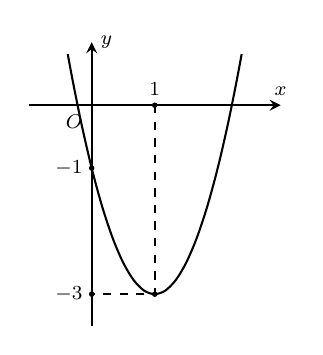
\begin{tikzpicture}[font=\footnotesize, >=stealth, x=0.8cm, y=0.8cm]
	\draw[->] (-1,0)--(3,0)node[above]{$x$};
	\draw[->] (0,-3.5)--(0,1)node[right]{$y$};
	\draw (0,0) node[below left]{$O$};
	\draw[dashed] (1,0) |- (0,-3);
	\begin{scope}
		\clip (-1,-3.5) rectangle (3,0.8);
		\draw[smooth] plot[domain=-1:3] (\x,{2*(\x)^2-4*(\x)-1});
	\end{scope}
	\fill[black]
		(0,-1) circle (1pt) node[left]{$-1$}
		(0,-3) circle (1pt) node[left]{$-3$}
		(1,0) circle (1pt) node[above]{$1$}
		(1,-3) circle (1pt)
		;
	\end{tikzpicture}}
	\par\shortans[]{$22$}
	\loigiai{
	Gọi $v(x)=mx^2+nx+q$ là hàm số vận tốc của vật ($m\ne 0$).
	\begin{itemize}
		\item Đồ thị hàm số đi qua điểm $(0;-1)$, suy ra $q=-1$.
		\item Đồ thị hàm số đi qua điểm $(1;-3)$, suy ra $m+n-1=-3 \Rightarrow m+n=-2$. \quad$(1)$
		\item Đồ thị hàm số có hoành độ đỉnh là $1$, suy ra $-\dfrac{n}{2m}=1 \Rightarrow 2m+n=0$. \quad$(2)$
	\end{itemize}
	Từ $(1)$ và $(2)$ ta có hệ phương trình $\heva{&m+n=-2 \\& 2m+n=0}\Leftrightarrow \heva{&m=2 \\& n=-4.} \quad\text{(thỏa mãn)}$\\
	Suy ra $v(x)=2x^2-4x-1$.\\
	Gọi $a(x)$ là hàm số gia tốc của vật, ta có $a(x)=v'(x)=4x-4$.\\
	Tại thời điểm vận tốc triệt tiêu, ta có $v(x)=0$ và $x> 0$.\\
	Ta có $v(x)=0 \Leftrightarrow 2x^2-4x-1=0 \Leftrightarrow \hoac{&x=\dfrac{2+\sqrt6}{2} \quad\text{(nhận)} \\& x=\dfrac{2-\sqrt6}{2}. \quad\text{(loại)}}$\\
	Khi đó $a\left(\dfrac{2+\sqrt6}{2}\right)=2\sqrt6$.\\
	Suy ra $a=2$; $b=6$. Vậy $2a+3b=22$.
	}
\end{bt}

\begin{bt}%[1D7H2-1]
% nguon: Archive/SP_DA_SauLuoi/1-TL-THPT-NguyenThiMinhKhai-TpHCM-HKII-NH23-24.tex #2471
%[Dự án đề kiểm tra Toán 11 HKII NH23-24- Ngô Tất Thành]%[THPT Nguyễn Thị Minh Khai]
	Tính đạo hàm của hàm số $y=\mathrm{e}^{\frac{1}{x}-\sqrt{x}+\log_5 x}$.
	\loigiai{
	Tập xác định của hàm số là $\mathscr{D}=(1;+\infty)$.\\
	Ta có $y'=\left(\dfrac{1}{x}-\sqrt{x}+\log_5 x \right)' \cdot \mathrm{e}^{\frac{1}{x}-\sqrt{x}+\log_5 x}=\left(-\dfrac{1}{x^2}-\dfrac{1}{2\sqrt{x}}+\dfrac{1}{x\ln 5} \right) \cdot \mathrm{e}^{\frac{1}{x}-\sqrt{x}+\log_5 x}$.
	}
\end{bt}

\begin{bt}%[1D7H3-1]
% nguon: Archive/SP_DA_SauLuoi/1-TL-THPT-NguyenThiMinhKhai-TpHCM-HKII-NH23-24.tex #2472
%[Dự án đề kiểm tra Toán 11 HKII NH23-24- Ngô Tất Thành]%[THPT Nguyễn Thị Minh Khai]
	Tính đạo hàm cấp hai của hàm số $y=2\cos x-x$.
	\loigiai{
	Ta có $y'=-2\sin x-1$, $y''=-2 \cos x$.
	}
\end{bt}

\begin{bt}%[1D7V2-4]
% nguon: Archive/SP_DA_SauLuoi/1-TL-THPT-NguyenThiMinhKhai-TpHCM-HKII-NH23-24.tex #2473
%[Dự án đề kiểm tra Toán 11 HKII NH23-24- Ngô Tất Thành]%[THPT Nguyễn Thị Minh Khai]
	Cho hàm số $y=f(x)=\dfrac{2x-1}{x+3}$ có đồ thị $(C)$. Viết phương trình tiếp tuyến $(\Delta)$ của đồ thị $(C)$ biết $(\Delta)$ song song với đường thẳng $d \colon y=7x+9$.
	\loigiai{
	Ta có $y'=f'(x)=\dfrac{7}{(x+3)^2}$.\\
	Gọi $x_0$ là hoành độ tiếp điểm.\\
	Vì tiếp tuyến $(\Delta)$ song song với đường thẳng $d \colon y=7x+9$ nên\\
	$f'(x_0)=7 \Leftrightarrow \dfrac{7}{(x_0+3)^2}=7 \Leftrightarrow (x_0+3)^2=1 \Leftrightarrow \hoac{&x_0=-2\\ &x_0=-4.}$\\
	Với $x_0=-2$ thì $(\Delta) \colon y=f(x_0)+f'(x_0)\cdot (x-x_0) = -5+7(x+2)=7x+9$ (loại).\\
	Với $x_0=-4$ thì $(\Delta) \colon y=f(x_0)+f'(x_0)\cdot (x-x_0) = 9+7(x+4)=7x+37$ (nhận).
	}
\end{bt}

\begin{bt}%[1D7H3-3]
% nguon: Archive/SP_DA_SauLuoi/1-TN-DS-TLN-THPT-LEHONGPHONG-THANHHOA-HKII-NH23-24.tex #2485
%%[Dự án đề kiểm tra Toán 11 HKI NH23-24-ĐÀO HOANG VŨ]%[THPT LÊ HỒNG PHONG - THANH HÓA]
Vị trí của một vật chuyển động thẳng đều được cho bởi phương trình $s=t^3-4t^2+4t$, trong đó $t$ tính bằng giây và $s$ tính bằng mét? Tính vận tốc của vật tại thời điểm $t=2$ giây.
\shortans[0]{$0$}
\loigiai{
Phương trình vận tốc của vật có dạng $v(t)=s'=3t^2-8t+4$.\\
Khi đó vận tốc của vật tại thời điểm $t=2$ giây bằng
\begin{center}
	$v(2)=3\cdot2^2-8\cdot2+4=0$.
\end{center}
Vậy vận tốc của vật tại thời điểm $t=2$ giây là $0$ m/s.
}
\end{bt}

\begin{bt}%[1D7H2-1]
% nguon: Archive/SP_DA_SauLuoi/1-TL-TN-THPT-AnThoi-BenTre-HKII-NH23-24.tex #2487
%[Dự án đề kiểm tra Toán 11 GHKI NH23-24- Nguyễn Mạnh Trung Anh]%[THPT AN THỚI- BẾN TRE]
Tính đạo hàm của các hàm số sau
\begin{multicols}{2}
	\begin{enumerate}
		\item $y=\cos\left(\dfrac{\pi}{6}-3x\right)$;
		\item $y=\dfrac{2x-3}{3x-1}$.
	\end{enumerate}
\end{multicols}
\loigiai{
\begin{enumerate}
	\item Hàm số $y=\cos\left(\dfrac{\pi}{6}-3x\right)$.\\
	Tập xác định $\mathscr{D}=\mathbb{R}$.\\
	Ta có $y'=\left[\cos\left(\dfrac{\pi}{6}-3x\right)\right]'=-\left(\dfrac{\pi}{6}-3x\right)'\sin\left(\dfrac{\pi}{6}-3x\right)=3\sin\left(\dfrac{\pi}{6}-3x\right)$.
	\item Hàm số $y=\dfrac{2x-3}{3x-1}$.\\
	Tập xác định $\mathscr{D}=\mathbb{R}\setminus\left\{\dfrac{1}{3}\right\}$.\\
	Ta có $y'=\left(\dfrac{2x-3}{3x-1}\right)'=\dfrac{2\cdot(-1)-3\cdot(-3)}{(3x-1)^2}=\dfrac{7}{(3x-1)^2}$.
\end{enumerate}
}
\end{bt}

\begin{bt}%[1D7H2-3]
% nguon: Archive/SP_DA_SauLuoi/1-TL-TN-THPT-AnThoi-BenTre-HKII-NH23-24.tex #2488
%[Dự án đề kiểm tra Toán 11 GHKI NH23-24- Nguyễn Mạnh Trung Anh]%[THPT AN THỚI- BẾN TRE]
	Viết phương trình tiếp tuyến của đồ thị hàm số $y=\dfrac{x^2+2x+3}{x-1}$ tại điểm có hoành độ bằng $-2$.
	\loigiai{
	Tập xác định $\mathscr{D}=\mathbb{R}$.\\
	Ta có 
	\begin{align*}
		y'=&\left(\dfrac{x^2+2x+3}{x-1}\right)'\\
		=&\dfrac{(x^2-2x+3)'(x-1)-(x-1)'(x^2+2x+3)}{(x-1)^2}\\
		=&\dfrac{(2x+2)(x-1)-(x^2+2x+3)}{(x-1)^2}\\
		=&\dfrac{x^2-2x-5}{(x-1)^2}.
	\end{align*}
	Khi đó $\heva{&y(-2)=-1\\&y'(-2)=\dfrac{1}{3}.}$\\
	Phương trình tiếp tuyến của đồ thị hàm số tại điểm có hoành độ bằng $-2$ là \[y=\dfrac{1}{3}(x+2)-1=\dfrac{1}{3}x-\dfrac{1}{3}.\] 	
	}
\end{bt}

\begin{bt}%[1D7H3-3]
% nguon: Archive/SP_DA_SauLuoi/1-TL-TN-DS-TLN-THPT-NguyenKhuyen-TpHCM-HKII-NH23-24.tex #2506
%[Dự án đề kiểm tra Toán 11 HKII NH23-24- Quan Ón]%[THPT Nguyễn Khuyến - Tp HCM]
	Một vật dao động điều hòa có phương trình $x = 2\sin \pi t$, với $x$ được tính bằng cm, $t$ tính bằng giây). Tính thời điểm đầu tiên vật có gia tốc lớn nhất. (kết quả ghi dưới dạng số thập phân)
	\loigiai{
		Ta có $v = x' = 2\pi\cos\left(\pi t\right)$.\\
		$a = v' = -2\pi^2\sin\left(\pi t\right)$.\\
		Vì $-1 \leq \sin\left(\pi t\right) \leq 1 \Leftrightarrow -2\pi^2 \leq -2\pi^2\sin\left(\pi t\right) \leq 2\pi^2$.\\
		Do đó, gia tốc lớn nhất là $2\pi^2$.\\
		Khi đó, ta có
		$$ -2\pi^2\sin\left(\pi t\right) = 2\pi^2 \Leftrightarrow \sin\left(\pi t\right) = -1 \Leftrightarrow \pi t = -\dfrac{\pi}{2} + k2\pi \Leftrightarrow t = -\dfrac{1}{2} + 2k, \quad (k \in \mathbb{Z}). $$
		Tại thời điểm đầu tiên nên $k = 1$, do đó $t = -\dfrac{1}{2} + 2\cdot 1 = \dfrac{3}{2}$ giây.\\
		Vây thời điểm đầu tiên vật có gia tốc lớn nhất là $\dfrac{3}{2} = 1{,}5$ giây.
	}
\end{bt}

\begin{bt}%[1D7H2-1]
% nguon: Archive/SP_DA_SauLuoi/1-TL-TN-DS-TLN-THPT-NguyenKhuyen-TpHCM-HKII-NH23-24.tex #2507
%[Dự án đề kiểm tra Toán 11 HKII NH23-24- Quan Ón]%[THPT Nguyễn Khuyến - Tp HCM]
	Tính đạo hàm của các hàm số sau
	\begin{listEX}[2]
		\item $y = \dfrac{x^3}{3} - 2x^2 - 3x + 1$;
		\item $y = \dfrac{\sin x}{1 - 2x}$;
		\item $y = (2x - 1)\sqrt{x^2 + x}$;
		\item $y = 3^{2x+1} + \log_3 \left(x^2 + 1\right)$.
	\end{listEX}
	\loigiai{
		\begin{enumerate}
			\item $y' = \left(\dfrac{x^3}{3} - 2x^2 - 3x + 1\right)' = x^2 - 4x - 3$.
			\item $y' = \left(\dfrac{\sin x}{1 - 2x}\right)' = \dfrac{\cos x(1 - 2x) - \sin x\cdot (-2)}{(1 - 2x)^2} = \dfrac{(1 - 2x)\cos x + 2\sin x}{(1 - 2x)^2}$.
			\item $y' = \left[(2x - 1)\sqrt{x^2 + x}\right]' = 2\sqrt{x^2 + x} + (2x - 1)\cdot\dfrac{2x + 1}{2\sqrt{x^2 + x}} = \dfrac{8x^2 + 4x - 1}{2\sqrt{x^2 + x}}$.
			\item $y' = \left(3^{2x+1} + \log_3 \left(x^2 + 1\right)\right)' = 2\cdot 3^{2x+1}\cdot \ln 3 + \dfrac{2x}{(x^2 + 1)\ln 3}$.
		\end{enumerate}
	}
\end{bt}

\begin{bt}%[1D7H2-3]
% nguon: Archive/SP_DA_SauLuoi/1-TN-DS-TLN-THPT-LuongTheVinh-HaNoi-HKII-NH23-24.tex #2514
%[Dự án đề kiểm tra Toán 11 GHKI NH23-24- Don Lee]%[THPT Lương Thế Vinh - Tp Hà Nội]
	Cho hàm số $y=\dfrac{1}{3}x^3-3x^2+7x+3$. Phương trình tiếp tuyến với đồ thị hàm số tại giao điểm của đồ thị với trục tung có dạng $y=ax+b$. Giá trị của $a+b$ bằng bao nhiêu?
	\loigiai{
		Ta có $y'=x^2-6x+7$.\\		
		Với $x=0$ thì $y(0)=3$ và $y'(0)=7$.\\
		Phương trình tiếp tuyến tại $x=0$ là $y=7x+3$.\\		
		Giá trị $a=7$; $b=3$. Vậy $a+b=10$.
	}
\end{bt}

\begin{bt}%[1D7V2-1]
% nguon: Archive/SP_DA_SauLuoi/1-TN-DS-TLN-THPT-LuongTheVinh-HaNoi-HKII-NH23-24.tex #2517
%[Dự án đề kiểm tra Toán 11 GHKI NH23-24- Don Lee]%[THPT Lương Thế Vinh - Tp Hà Nội]
	Cho hai hàm số $f(x)=\dfrac{30x^3}{x^2+2}$ và $g(x)=\dfrac{60x}{x^2+2}$. Biết $f'(x_0)=12$ giá trị của $g'(x_0)$ bằng bao nhiêu?
	\loigiai{
		Ta có $f'(x)=\dfrac{(90x^2)(x^2+2)-(30x^3)(2x)}{(x^2+2)^2}=\dfrac{30x^2(x^2+6)}{(x^2+2)^2}$.\\
		Có $f'(x_0)=12 \Rightarrow \dfrac{30x_0^2(x_0^2+6)}{(x_0^2+2)^2}=12 \Leftrightarrow 30+\dfrac{60x_0^2-120}{(x_0^2+2)^2}=12 \Leftrightarrow -\dfrac{60x_0^2-120}{(x_0^2+2)^2}=18$.\\
		Lại có $g'(x)=\dfrac{60(x^2+2)-60x(2x)}{(x^2+2)^2}=\dfrac{120-60x^2}{(x^2+2)^2}$.\\
		Suy ra $g'(x_0)=-\dfrac{60x_0^2-120}{(x_0^2+2)^2}=18$.
	}
\end{bt}

\begin{bt}%[1D7H1-4]
% nguon: Archive/SP_DA_SauLuoi/1-TN-DS-TLN-SGD-NamDinh-HKII-NH23-24.tex #2527
%[Dự án đề kiểm tra Toán 11 HKII NH23-24 - Thành Đức Trung]%[Sở Nam Định]
Một chất điểm chuyển động với phương trình $s(t)=t^3+3t^2-t+2$ ($s(t)$ là quãng đường tính bằng mét, $t$ là thời gian tính bằng giây). Vận tốc tức thời của chất điểm tại thời điểm $t=2$ giây là $a$ m/s. Tìm $a$.
\shortans{$23$}
\loigiai
{
Phương trình vận tốc tức thời của chất điểm là $v(t)=s'(t)=3t^2+6t-1$. \\
Tại thời điểm $t=2$ giây, vận tốc tức thời của chất điểm là $v(2)=3\cdot2^2+6\cdot 2-1=23$ (m/s).
}
\end{bt}

\begin{bt}%[1D7H2-1]
% nguon: Archive/SP_DA_SauLuoi/1-TL-TN-THPT-Chuyen-LeQuyDon-NinhThuan-HKII-NH23-24.tex #2534
%[Dự án đề kiểm tra Toán 11 CKII NH23-24-Đợt 16-Lê Hữu Kiệt]%[THPT Chuyên Lê Quý Đôn- Ninh Thuận]
	Cho hàm số $y=f(x)=\mathrm{e}^{-2x}\sin 2x$. Tính $f'(x)$.
	\loigiai{
	Ta có\\
	$f'(x)= \left(\mathrm{e}^{-2x}\right)' \cdot \sin2x + \mathrm{e}^{-2x}\cdot (\sin 2x)'  = -2\mathrm{e}^{-2x}\sin2x + 2\mathrm{e}^{-2x}\cos2x.$
	}
\end{bt}

\begin{bt}%[1D7H2-8]
% nguon: Archive/SP_DA_SauLuoi/1-TL-TN-THPT-Chuyen-LeQuyDon-NinhThuan-HKII-NH23-24.tex #2535
%[Dự án đề kiểm tra Toán 11 CKII NH23-24-Đợt 16-Lê Hữu Kiệt]%[THPT Chuyên Lê Quý Đôn- Ninh Thuận]
	\immini[thm]
	{Một vật chuyển động trong $4$ giờ với vận tốc $v$ phụ thuộc vào thời gian $t$ và có đồ thị vận tốc như hình bên. Trong khoảng thời gian $4$ giờ kể từ khi bắt đầu chuyển động, đồ thị đó là một phần của đường parabol có đỉnh $I\left( \dfrac{5}{2};\,-\dfrac{9}{4} \right)$ và có trục đối xứng song song trục tung. Tính gia tốc của vật lúc $t=3$ giờ.}
	{\begin{tikzpicture}[font=\footnotesize, >=stealth, x=0.6cm, y=0.6cm]
	\draw[->] (-0.5,0)--(6,0)node[above]{$t$ (giờ)};
	\draw[->] (0,-3)--(0,5)node[left]{$v$ (km/giờ)};
	\draw (0,0) node[below left]{$O$};
	\draw[dashed] (5/2,0) |- (0,-9/4);
	\begin{scope}
		\clip (-0.5,-3) rectangle (5.5,4.8);
		\draw[smooth] plot[domain=0:4] (\x,{(\x)^2-5*(\x)+4});
	\end{scope}
	\foreach \x in {(5/2,0), (0,4), (0,-9/4), (5/2,-9/4)}{\fill[black] \x circle (1pt);}
	\draw (0,4)node[left]{$4$} (0,-9/4)node[left]{$-\dfrac{9}{4}$} (5/2,0)node[above]{$\dfrac{5}{2}$} (5/2,-9/4)node[below]{$I$};
	\end{tikzpicture}}
	\loigiai{
	Gọi $v(t)=at^2+bt+c$ ($a> 0$) là hàm số vận tốc cần tìm (đơn vị: km/giờ). Ta có
	\begin{itemize}
		\item Đồ thị hàm số đi qua điểm $(0;\,4)$, suy ra $c=4$;
		\item Hoành độ đỉnh $I$ là $-\dfrac{b}{2a}=\dfrac{5}{2} \Leftrightarrow b=-5a$; \quad$(1)$
		\item Tung độ đỉnh $I$ là $-\dfrac{b^2-4ac}{4a}=-\dfrac{9}{4} \Leftrightarrow b^2-16a=9a \Leftrightarrow b^2-25a=0$. \quad$(2)$
	\end{itemize}
	Thay $(1)$ vào $(2)$ ta được
	\allowdisplaybreaks
	\begin{eqnarray*}
		&& (-5a)^2-25a=0 \\
		&& 25a^2-25a=0 \\
		&& a=1 \quad\text{hoặc} \quad a=0.
	\end{eqnarray*}
	Vì $a>0$ nên ta nhận $a=1$. Khi đó $b=-5\cdot1=-5$.\\
	Suy ra $v(t)=t^2-5t+4$.\\
	Gọi $a(t)$ là gia tốc của vật (đơn vị: km/giờ$^2$), ta có $a(t)=v'(t)=2t-5$.\\
	Khi đó, gia tốc của vật lúc $t=3$ giờ là $a(3)=1$ (km/giờ$^2$).
	}
\end{bt}

\begin{bt}%[1D7N2-1]
% nguon: Archive/SP_DA_SauLuoi/1-TL-TN-THPT-HungVuong-HKII-TpHCM-NH23-24.tex #2549
%[Dự án đề kiểm tra Toán 11 HKII NH23-24- Nguyễn Tấn Linh]%[THPT Hùng Vương - Tp HCM]
	Tính đạo hàm của hàm số sau
	\[y=x^4+\sqrt{x}-\dfrac{1}{x}+2024.\]
	\loigiai
	{
		Ta có $y'=4x^3+\dfrac{1}{2\sqrt{x}}+\dfrac{1}{x^2}$.
	}
\end{bt}

\begin{bt}%[1D7H2-1]
% nguon: Archive/SP_DA_SauLuoi/1-TL-THPT-NguyenTatThanh-HCM-HKII-NH23-24.tex #2553
%[Dự án đề kiểm tra Toán 11 HKII NH23-24- Trần Xuan Hòa]%[THPT NguyenTatTHanh]
	Tính đạo hàm của các hàm số $y=\log_3(\tan x)$.
	\loigiai{
	Ta có $y'=\dfrac{(\tan x)'}{\tan x\cdot \ln 3}=\dfrac{1+\tan ^2 x}{\tan x \cdot \ln 3}$.
	}
\end{bt}

\begin{bt}%[1D7H2-1]
% nguon: Archive/SP_DA_SauLuoi/1-TL-THPT-NguyenTatThanh-HCM-HKII-NH23-24.tex #2554
%[Dự án đề kiểm tra Toán 11 HKII NH23-24- Trần Xuan Hòa]%[THPT NguyenTatTHanh]
	Tính đạo hàm của các hàm số $y=e^x \cos x$.
	\loigiai{
		Ta có $y'=(e^x)\cdot \cos x+(e^x)\cdot (\cos x)'=e^x(\cos x-\sin x)$.
	}
\end{bt}

\begin{bt}%[1D7H2-1]
% nguon: Archive/SP_DA_SauLuoi/1-TL-THPT-NguyenTatThanh-HCM-HKII-NH23-24.tex #2555
%[Dự án đề kiểm tra Toán 11 HKII NH23-24- Trần Xuan Hòa]%[THPT NguyenTatTHanh]
	Tính đạo hàm của các hàm số $y=\dfrac{x^2}{\sin x}$.
	\loigiai{
		Ta có $y'=\dfrac{(x^2)'\cdot (\sin x)-(\sin x)'\cdot x^2}{\sin^2x}=\dfrac{2 x \sin x-x^2 \cos x}{\sin ^2 x}$.
	}
\end{bt}

\begin{bt}%[1D7H2-4]
% nguon: Archive/SP_DA_SauLuoi/1-TL-THPT-NguyenTatThanh-HCM-HKII-NH23-24.tex #2556
%[Dự án đề kiểm tra Toán 11 HKII NH23-24- Trần Xuan Hòa]%[THPT NguyenTatTHanh]
	Viết phương trình tiếp tuyến của đường cong $(C)\colon y=\sqrt{x}$, biết tiếp tuyến có hệ số góc bằng $2$.
	\loigiai{
		Ta có $y'=\dfrac{1}{2 \sqrt{x}}$ và $y'=2 \Leftrightarrow x=\dfrac{1}{16}$.\\
		Phương trình tiếp tuyến là $y=2 x+\dfrac{1}{8}$.
	}
\end{bt}

\begin{bt}%[1D7H3-1]
% nguon: Archive/SP_DA_SauLuoi/1-TL-TN-DS-THPT-ChuyenTranPhu-HaiPhong-HKII-NH23-24.tex #2564
%[Dự án đề kiểm tra Toán 11 HK2 NH23-24 - Phan Anh]%[THPT Chuyên Trần Phú - Hải Phòng]
Cho hàm số $f(x)=\dfrac{x^2+x+1}{x+1}$. Tập nghiệm của bất phương trình $f''(x)>0$ có bao nhiêu giá trị nguyên dương $x\le2024$?
\loigiai{Ta có $f(x)=\dfrac{x^2+x+1}{x+1}=\dfrac{x(x+1)+1}{x+1}=x+\dfrac{1}{x+1}$, suy ra 
\[f'(x)=1-\dfrac{1}{(x+1)^2},\,f''(x)=\dfrac{2}{(x+1)^3}.\]
Do đó nên $f''(x)>0\Leftrightarrow\dfrac{2}{(x+1)^3}>0\Leftrightarrow x+1>0\Leftrightarrow x>-1$.\\
Do $x$ là số nguyên dương và $x\le2024$ nên $x\in\{1;2;\ldots;2024\}$.\\
Vậy có $2024$ giá trị $x$ thỏa mãn yêu cầu bài toán.}
\end{bt}

\begin{bt}%[1D7H2-1]
% nguon: Archive/SP_DA_SauLuoi/1-TL-TN-DS-THPT-ChuyenTranPhu-HaiPhong-HKII-NH23-24.tex #2565
%[Dự án đề kiểm tra Toán 11 HK2 NH23-24 - Phan Anh]%[THPT Chuyên Trần Phú - Hải Phòng]
Cho hàm số $y=\dfrac{x^2+x-2}{x^2-x+3}$. Biết $y'=\dfrac{-2x^2+ax+b}{\left(x^2-x+3\right)^2}$. Tính $P=a\cdot b$.
\loigiai{Ta có $y=\dfrac{x^2+x-2}{x^2-x+3}$ nên
\[y'=\dfrac{(2x+1)\left(x^2-x+3\right)-\left(x^2+x-2\right)(2x-1)}{\left(x^2-x+3\right)^2}=\dfrac{-2x^2+10x+1}{\left(x^2-x+3\right)^2}.\]
Từ đó ta có $a=10$ và $b=1$, suy ra $P=a\cdot b=10$.}
\end{bt}

\begin{bt}%[1D7N2-4]
% nguon: Archive/SP_DA_SauLuoi/1-TL-THPT-PTNK-TpHCM-HKII-NH23-24.tex #2577
%[Dự án A - đợt 15, Nguyễn Quang Hiệp]%[Đề kiểm tra học kỳ 2, THPT PTNK, TP HCM, năm học 2023 2024]
Cho $(C)\colon y=x^3-6 x^2-7 x+5$. Viết phương trình tiếp tuyến $\Delta$ của đồ thị $(C)$. Biết $\Delta \parallel  d\colon y=5-7 x$.	
	\loigiai{
	Ta có $y=x^3-6 x^2-7 x+5\Rightarrow y'=3x^2-12x-7$.\\
	Gọi $M(x_0;y_0)$ là tiếp điểm. Khi đó phương trình đường thẳng $\Delta$ có dạng
	\[\Delta\colon y=f'(x_0)(x-x_0)+y_0.\]
	Lại có $\Delta \parallel d$, suy ra \allowdisplaybreaks
	\begin{eqnarray*}
	&&f'(x_0)=-7\\
	&\Rightarrow &3x_0^2-12x_0-7=-7\\
	&\Leftrightarrow &3x_0^2-12x_0=0\\
	&\Leftrightarrow &\hoac{&x_0=0\\&x_0=4.}
	\end{eqnarray*}	
	\begin{itemize}
	\item Với $x_0=0\Rightarrow y_0=5$. Khi đó đường thẳng $\Delta$ có phương trình là
	\[y=-7x(x-0)+5\Leftrightarrow y=-7x+5.\]
	Do đó $\Delta$ trùng với $d$.
	\item Với $x_0=-4\Rightarrow y_0=-127$. Khi đó đường thẳng $\Delta$ có phương trình là
	\allowdisplaybreaks
	\begin{eqnarray*}
	y=-7(x+4)-127\Leftrightarrow y=-7x-155.
	\end{eqnarray*}		
	\end{itemize}	
	}
\end{bt}

\begin{bt}%[1D7H3-2]
% nguon: Archive/SP_DA_SauLuoi/1-TL-THPT-PTNK-TpHCM-HKII-NH23-24.tex #2578
%[Dự án A - đợt 15, Nguyễn Quang Hiệp]%[Đề kiểm tra học kỳ 2, THPT PTNK, TP HCM, năm học 2023 2024]
Cho hàm số $y=2 \sin x+4 \cos x$. Chứng minh: $3 y+y'+y''=10 \cos x$	
	\loigiai{
	Ta có \allowdisplaybreaks
	\begin{eqnarray*}
	&&y=2 \sin x+4 \cos x\\
	&\Rightarrow& y'=2\cos x -4\sin x\\
	&\Rightarrow &y''=-2\sin x -4 \cos x.
	\end{eqnarray*}
	Do đó \allowdisplaybreaks
	\begin{eqnarray*}
	&&3 y+y'+y''\\
	&=&3\left(2 \sin x+4 \cos x\right)+2\cos x -4\sin x+-2\sin x -4 \cos x\\
	&=&6\sin x +12\cos x -6\sin x -2\cos x\\
	&=&10\cos x.
	\end{eqnarray*}
	}
\end{bt}

\begin{bt}%[1D7H3-3]
% nguon: Archive/SP_DA_SauLuoi/1-TL-THPT-PTNK-TpHCM-HKII-NH23-24.tex #2579
%[Dự án A - đợt 15, Nguyễn Quang Hiệp]%[Đề kiểm tra học kỳ 2, THPT PTNK, TP HCM, năm học 2023 2024]
\immini{
Một con lắc lò xo dao động điều hòa theo phương ngang trên mặt phẳng không ma sát như hình vẽ, có phương trình chuyển động $x=4 \sin 2 t$, trong đó $t$ tính bằng giây và $x$ tính bằng centimét. Biết vận tốc và gia tốc của con lắc tại thời điểm $t$ lần lượt là $v(t)=x'(t)$ và $a(t)=x''(t)$. Tính vận tốc và gia tốc của con lắc tại thời điểm $t=\dfrac{\pi}{3}$.	
}{
\begin{tikzpicture}[>=stealth,line join=round,line cap=round,font=\footnotesize,scale=1]
	% Supporting structure
	\tikzset{declare function={a=3.2;h=2.5;}}
	\fill [pattern = north west lines] (0,0)rectangle(0.2,h);
	\draw[ultra thick] (0.2,0)coordinate (A) --(0.2,h)coordinate (B)
	($(A)!.25!(B)$)coordinate (M);
	;
	\draw[->,thick] (0,0)--(5,0)node[below]{$x$};
	\filldraw[pattern=north east lines,thick] (a,0)rectangle(a+.8,1.25) (a,0)--(a+.8,0)node[below,midway]{$x$};
	% Spring 
	\draw[decoration={coil,	aspect=0.1,	segment length=1mm, amplitude=2.5mm, 	pre length=3mm,	post length=3mm},decorate,thick] (M) -- ++(0:3) 
; 
	\draw (2.5,0)coordinate (O)circle(1pt)node[below]{$O$};
	\draw[->] (2.5,h-.3)node[above]{Vị trí cân bằng}--(2.5,1);
	
\end{tikzpicture}
}
\loigiai{
Ta có $x(t)=4 \sin 2t\Rightarrow v(t)=x'(t)=8\cos 2t$.\\
Do đó vận tốc của vật tại thời điểm $t=\dfrac{\pi}{3}$ là 
\allowdisplaybreaks
\begin{eqnarray*}
v\left(\dfrac{\pi}{3}\right)=8\cos\left(2\cdot \dfrac{\pi}{3}\right)=4\,(\text{m/s}).
\end{eqnarray*}	
Ta có $a(t)=x''(t)=-16\sin 2t$.\\
Do đó gia tốc của vật tại thời điểm $t=\dfrac{\pi}{3}$ là 
\allowdisplaybreaks
\begin{eqnarray*}
a\left(\dfrac{\pi}{3}\right)=-16\sin\left(2\cdot \dfrac{\pi}{3}\right)=-8\sqrt{3}\,(\text{m/s}^2).
\end{eqnarray*}
}
\end{bt}

\begin{bt}%[1D7H2-1]
% nguon: Archive/SP_DA_SauLuoi/1-TL-TN-DS-THPT-BaoLoc-LamDong-HKII-NH23-24.tex #2600
%[Dự án đề kiểm tra Toán 11 GHKI NH23-24- Phan Trung Hiếu]%[THPT Bảo Lộc- Lâm Đồng]
	\begin{enumerate}
		\item Tính đạo hàm của hàm số $y=x^4+2\sin x - \mathrm{e}^{5x}$.
		\item Giải phương trình $\log_2x+\log_2(x-1)=1$.
	\end{enumerate}
	\loigiai{
		\begin{enumerate}
			\item $y'=4x^3+2\cos x - 5\mathrm{e}^{5x}$.
			\item Điều kiện: $\heva{&x>0\\&x-1>0}\Leftrightarrow x>1$.
			Ta có
			\begin{equation*}
				\log_2x(x-1)=1\Leftrightarrow x^2-x-2=0\Leftrightarrow\heva{&x=-1\,\text{(Loại)}\\&x=2\,\text{(Nhận)}.}
			\end{equation*}
		\end{enumerate}
	}
	
\end{bt}

\begin{bt}%[1D7H2-8]
% nguon: Archive/SP_DA_SauLuoi/1-TN-DS-TLN-THPT-TruongVinhKy-BenTre-HKII-2023-2024.tex #2609
%[Dự án đề kiểm tra Toán 11 HKII NH23-24- Nhật Thiện]%[THPT Trương Vĩnh Ký - Bến Tre]
	Kính viễn vọng trong không gian Hubble được triển khai vào ngày $24$ tháng $4$ năm $1990$, bởi tàu con thoi Discovery. Vận tốc của tàu con thoi trong nghiệm vụ này từ khi xuất phát tại $t=0$ (s) cho đến khi tên lửa đẩy nhiên liệu rắn bị loại bỏ ở $t=126$ (s), được xác định theo phương trình sau
	$$v(t)=0{,}001302 t^3-0{,}09029 t^2+23{,}61 t-3{,}083\text{ (ft/s)}.$$
	(\textit{Nguồn: James Stewart, Calculus})\\
	Tính gia tốc tức  thời của tàu con thoi tại thời điểm $t=100$ (s) (làm tròn kết quả đến hàng phần mười).
	\shortans[]{$44{,}6$}
	\loigiai{
	Gia tốc của tàu con thoi 
	$$a(t)=v'(t)=0{,}003906 t^2-0{,}18058 t+23{,}61.$$
	Gia tốc tức thời của tàu con thoi tại thời điểm $t=100$ là $a(100)\approx 44{,}6$.
}
\end{bt}

\begin{bt}%[1D7H2-3]
% nguon: Archive/SP_DA_SauLuoi/1-TN-DS-TLN-THPT-TruongVinhKy-BenTre-HKII-2023-2024.tex #2610
%[Dự án đề kiểm tra Toán 11 HKII NH23-24- Nhật Thiện]%[THPT Trương Vĩnh Ký - Bến Tre]
	Cho hàm số $f(x)=\dfrac{x^2-4x-5}{x-2}$.
	\begin{enumerate}
		\item Tính $f'(x)$ và giải phương trình $f'(x)=0$.
		\item Viết phương trình tiếp tuyến của đồ thị hàm số tại điểm có hoành độ $x=3$.
	\end{enumerate}
\loigiai{
\begin{enumerate}
	\item Ta có $f'(x)=\dfrac{(2x-4)(x-2)-(x^2-4x-5)}{(x-2)^2}=\dfrac{x^2-4x+13}{(x-2)^2}$\\
	Khi đó $f'(x)=0\Leftrightarrow x^2-4x+13=0$ (phương trình vô nghiệm).\\
	\item Với $x=3\Rightarrow y=-8$.\\	
	Phương trình tiếp tuyến của đồ thị hàm số tại điểm có hoành độ $x=3$ là
	$$y=y'(3)\cdot (x-3)-8=10(x-3)-8=10x-38.$$
\end{enumerate}
}
\end{bt}

\begin{bt}%[1D7H3-2]
% nguon: Archive/SP_DA_SauLuoi/1-TN-DS-TLN-THPT-TruongVinhKy-BenTre-HKII-2023-2024.tex #2612
%[Dự án đề kiểm tra Toán 11 HKII NH23-24- Nhật Thiện]%[THPT Trương Vĩnh Ký - Bến Tre]
	Cho hàm số $y=x\sin x$. Giải phương trình $y''+y=1$.
	\loigiai{
	Ta có $y'=x'\cdot \sin x+x\cdot (\sin x)'=\sin x+x\cdot \cos x$.\\
	Khi đó $y''=\cos x+\cos x-x\sin x=2\cos x-x\sin x$.\\
	Xét phương trình 
	\begin{eqnarray*}
		&&y''+y=1\Leftrightarrow 2\cos x-x\sin x+x\sin x=1\\
		&\Leftrightarrow& \cos x=\dfrac{1}{2}=\cos \dfrac{\pi}{3}\\
		&\Leftrightarrow& x=\pm\dfrac{\pi}{3}+k2\pi,\ (k\in \mathbb{Z}).
	\end{eqnarray*}
}
\end{bt}

\begin{bt}%[1D7H2-1]
% nguon: Archive/SP_DA_SauLuoi/1-TL-TN-THPT-ChauVanLiem-HKII-NH23-24.tex #2613
%[Dự án đề kiểm tra Toán 11 HKII NH23-24- Phạm Văn Long]%[THPT Châu Văn Liêm - Cần Thơ]
	Tính đạo hàm của các hàm số sau:
	\begin{listEX}[2]
		\item $y=\mathrm{e}^x+2x$
		\item $y=\sqrt{x^2+2}$.
	\end{listEX}
	\loigiai{
	\begin{listEX}[2]
		\item $y'=\mathrm{e}^x+2$.
		\item $y'=\dfrac{x}{\sqrt{x^2+2}}$.
	\end{listEX}
	}
\end{bt}

\begin{bt}%[1D7H2-3]
% nguon: Archive/SP_KhoLatex/ID6_old/DeThamKhao-02.tex #3213
%[Dự án ĐGNL-ĐGTD-2022 GĐ1]%[Lê Minh Thiện Anh]
	Cho hàm số $y = x^4 - 4x^2 + 4$ có đồ thị $(C)$. Viết phương trình tiếp tuyến với $(C)$ tại điểm $M(1;1)$.\\
	\textit{Kết quả:} \tikz\draw (0,0) rectangle (3,0.6);
	\loigiai{
		Ta có: $y' = 4x^3 - 8x$, $y'(1) = -4$. \\
		Vậy phương trình tiếp tuyến của đồ thị $(C)$ tại $M(1;1)$ là: $y = y'(1)(x - 1) + 1 \Leftrightarrow y  = -4x + 5$.
	}
\end{bt}

\begin{bt}%[1D7V2-7]
% nguon: Archive/SP_KhoLatex/ID6_old/DeThamKhao-03.tex #3282
%[Dự án ĐGNL-ĐGTD-2022 GĐ1]%[Duong Xuan Loi]
	Cho số nguyên dương $n$ thỏa mãn $\mathrm{C}_n^0+2\mathrm{C}_n^1+3\mathrm{C}_n^2+\cdots+(n+1)\mathrm{C}_n^n=131072$. Tìm $n$.
	
	\textit{Kết quả:} \tikz\draw (0,0) rectangle (3,0.6);
	\loigiai{
		Xét $(1+x)^n=\mathrm{C}_n^0+\mathrm{C}_n^1x+\mathrm{C}_n^2x^2+\cdots+\mathrm{C}_n^nx^n$ $\quad (1)$.\\
		Nhân hai vế của $(1)$ cho $x$ ta được $(1+x)^nx=\mathrm{C}_n^0x+\mathrm{C}_n^1x^2+\mathrm{C}_n^2x^3+\cdots+\mathrm{C}_n^nx^{n+1}$ $\quad (2)$.\\
		Lấy đạo hàm hai vế của $(2)$ theo ẩn $x$ ta được
		$$n(1+x)^{n-1}x+(1+x)^n=\mathrm{C}_n^0+2\mathrm{C}_n^1x+3\mathrm{C}_n^2x^2+\cdots+(n+1)\mathrm{C}_n^nx^n \quad (3)$$
		Thay $x=1$ vào $(3)$, ta được 
		$n\cdot2^{n-1}+2^n=\mathrm{C}_n^0+2\mathrm{C}_n^1+3\mathrm{C}_n^2+\cdots+(n+1)\mathrm{C}_n^n
		\Leftrightarrow n\cdot2^{n-1}+2^n=131072$.\\
		Nếu $n > 10$ thì  $n\cdot2^{n-1}+2^n>10\cdot2^9+2^{10}=6144$.\\
		Nếu $n < 15$ thì $n\cdot2^{n-1}+2^n<15\cdot2^{14}+2^{15}=278528$.\\
		Vậy $n\in\left[10;15\right) $.\\
		\textbf{Cách khác:}
		Xét $x(1+x)^n= \mathrm{C}_n^0 x  + \mathrm{C}_n^1 x^2 + \mathrm{C}_n^2 x^3 +\cdots + \mathrm{C}_n^n x^{n+1}$ \quad(*)\\
		Đạo hàm $2$ vế của (*), ta được:
		$$(1+x)^n+x\cdot n\cdot (1+x)^{n-1}= \mathrm{C}_n^0  +2 \mathrm{C}_n^1 x + 3\mathrm{C}_n^2 x^2 +\cdots + (n+1)\mathrm{C}_n^n x^n  \quad(\ast\ast)$$
		Cho $x=1$: $(\ast\ast)\Leftrightarrow 2^n+n\cdot 2^{n-1}=\mathrm{C}_n^0  + 2\mathrm{C}_n^1 + 3\mathrm{C}_n^2 +\cdots + (n + 1)\mathrm{C}_n^n$.\\
		Yêu cầu bài toán tương đương với $2^n+n\cdot 2^{n-1}=131072 \quad(1)$\\
		\textbf{Nhận xét:}
		$(1)\Leftrightarrow n+2=2^{18-n}<22 \Rightarrow  2^{18-n}\leq 2^4 $
		hay $n\geq 14$.\\
		Mặt khác $(1)$ có nghiệm $n=14$.
	}
\end{bt}

\begin{bt}%[1D7H2-4]
% nguon: Archive/SP_KhoLatex/ID6_old/bai8.1.tex #3448

	Cho đồ thị hàm số $(C)\colon y= \dfrac {2x-1}{x+4}$. Viết phương trình tiếp tuyến của $(C)$ biết tiếp tuyến có hệ số góc bằng $9$.
	%\dapso{$y=9x+20$, $y=9x+56$}
	\loigiai
	{$y= \dfrac {2x-1}{x+4} \Rightarrow y'= \dfrac {9}{(x+4)^2}.$ Gọi hoành độ tiếp điểm là $x_0$ ($x_0\neq -4$).\\
		Theo đề bài, ta có $y'(x_0)=9\Leftrightarrow\dfrac {9}{(x_0+4)^2} =9\Leftrightarrow\hoac{&x_0=-3\\&x_0=-5.}$\\
		TH1: $x_0=-3 \Rightarrow y(-3)=-7$. Suy ra phương trình tiếp tuyến là $y=9(x+3)-7 \Leftrightarrow y=9x+20$.\\
		TH2: $x_0=-5 \Rightarrow y(-5)=11$. Suy ra phương trình tiếp tuyến là $y=9(x+5)+11\Leftrightarrow y=9x+56$.
	}
\end{bt}

\begin{bt}%[1D7H2-4]
% nguon: Archive/SP_KhoLatex/ID6_old/bai8.1.tex #3449

	Cho hàm số $y = \dfrac{x+1}{x+3}$ có đồ thị $(C)$. Viết phương trình tiếp tuyến $d$ của đồ thị, biết $d$ song song với đường thẳng $\Delta:\, y = 2x + 3$.
	%\dapso{$y = 2x + 11$, $y = 2x - 5$}
	\loigiai{ Đặt $f(x) = \dfrac{x+1}{x+3}$, ta có $f'(x) = \dfrac{2}{(x+3)^2}$. \\
		Do tiếp tuyến $d$ song song với đường thẳng $\Delta:\, y = 2x + 3$ nên hệ số góc của tiếp tuyến bằng $2$. \\
		Gọi $M(x_0;\, f(x_0)) \in (C)$ là tiếp điểm của tiếp tuyến $d$ với đồ thị $(C)$. Khi đó phương trình tiếp tuyến $d$ là
		$$ y = f'(x_0) (x - x_0) + f(x_0).$$
		Hệ số góc của tiếp tuyến bằng 2 $\Leftrightarrow f'(x_0) = 2 \Leftrightarrow \dfrac{2}{(x_0 + 3)^2} = 2 \Leftrightarrow \hoac{& x_0 = - 4 \\ & x_0 = - 2.}$ \\
		Với $x_0 = - 4$ thì $f(x_0) = 3$, phương trình tiếp tuyến là $y = 2(x + 4) + 3$ hay $y = 2x + 11$ (thỏa mãn song song với $\Delta$). \\
		Với $x_0 = - 2$ thì $f(x_0) = -1$, phương trình tiếp tuyến là $y = 2(x - 2) - 1 $ hay $y = 2x - 5$ (thỏa mãn song song với $\Delta$). \\
	}
\end{bt}

\begin{bt}%[1D7H2-4]
% nguon: Archive/SP_KhoLatex/ID6_old/bai8.1.tex #3450

	Cho đường cong $(C)\colon y=f(x)=x^3+3x^2-4x-2$. Viết phương trình tiếp tuyến của $(C)$, biết tiếp tuyến vuông góc với đường thẳng $(d)\colon y=\dfrac{1}{4}x+\dfrac{1}{4}$.
	%\dapso{(tt)$\colon y=-4x-2$ và (tt)$\colon y=-4x+2$}
	\loigiai{
		Gọi $M(x_0;y_0)$ là tiếp điểm. Tiếp tuyến vuông góc với đường thẳng $(d)\colon y=\dfrac{1}{4}x+\dfrac{1}{4}$ suy ra
		$$f'(x_0)\cdot \dfrac{1}{4}=-1\Leftrightarrow f'(x_0)=-4\Leftrightarrow 3x_0^2+6x_0-4=-4\Leftrightarrow \hoac{&x_0=0\\ &x_0=-2.}$$
		Với $x_0=0\Rightarrow y_0=-2\Rightarrow$ (tt)$\colon y=-4(x-0)-2=-4x-2$.\\
		Với $x_0=-2\Rightarrow y_0=10\Rightarrow$ (tt)$\colon y=-4(x+2)+10=-4x+2$.
	}
\end{bt}

\begin{bt}%[1D7N2-3]
% nguon: Archive/SP_KhoLatex/ID6_old/17-OT-TiepTuyen.tex #3732
%[ĐGNL-ĐGTD-2022]%[Lương Như Quỳnh]
Viết phương trình tiếp tuyến của đồ thị hàm số $y =f(x)= -x^3 + x$ tại điểm $M(-2;6)$.
	\loigiai{
		Ta có $f'(x) = -3x^2 + 1$.\\
		Vì $d$ có tiếp điểm là $M(-2;6)$ nên $d$ hệ số góc tiếp tuyến $k = f'(-2) = -3\cdot (-2)^2 + 1 = -11$.\\
		Phương trình tiếp tuyến của đồ thị hàm số đã cho tại điểm $M(-2;6)$ là $(d)\colon y = -11x - 16$.
	}
\end{bt}

\begin{bt}%[1D7H2-3]
% nguon: Archive/SP_KhoLatex/ID6_old/17-OT-TiepTuyen.tex #3733
%[ĐGNL-ĐGTD-2022]%[Lương Như Quỳnh]
	Cho hàm số $y=x^3+3x^2-9x$ có đồ thị $(C)$. Viết phương trình tiếp tuyến với đồ thị hàm số $(C)$ tại điểm có hoành độ bằng  $2$.
	\loigiai{
Ta có $y'=3x^2+6x-9$, $y(2)=2$, $y'(2)=15$.\\
Vậy phương trình tiếp tuyến với đồ thị hàm số $(C)$ tại điểm có hoành độ bằng  $2$ là
\[y=y'(2)(x-2)+y(2)\Leftrightarrow y=15(x-2)+2\Leftrightarrow y=15x-28.\]
	}
\end{bt}

\begin{bt}%[1D7H2-3]
% nguon: Archive/SP_KhoLatex/ID6_old/17-OT-TiepTuyen.tex #3734
%[ĐGNL-ĐGTD-2022]%[Lương Như Quỳnh]
	Cho hàm số $y=x^3-3x+1$ có đồ thị là $\left( C \right)$. Viết phương trình tiếp tuyến của $\left( C \right)$ tại điểm có tung độ bằng $3$.
	\loigiai{
		Ta có ${y}'=3x^2-3$.\\
		Gọi $M\left( {x_0};\,y_0 \right)$ là tiếp điểm.\\
		Với $y_0=3\Leftrightarrow x_0^3-3x_0-2=0\Leftrightarrow\hoac{&x_0=2\\&x_0=-1.}$
		\begin{itemize}
			\item ${x_0}=-1\Rightarrow {y}'(-1)=0$. Phương trình tiếp tuyến tại điểm $(-1; 3)$ là  $y=3$.
			\item $x_0 = 2 \Rightarrow y'(2) = 9$. Phương trình tiếp tuyến tại điểm $(2; 3)$ là $y = 9(x-2)+ 3$ hay $y = 9x-15$.
		\end{itemize}
	}
\end{bt}

\begin{bt}%[1D7H2-4]
% nguon: Archive/SP_KhoLatex/ID6_old/17-OT-TiepTuyen.tex #3735
%[ĐGNL-ĐGTD-2022]%[Lương Như Quỳnh]
Viết phương trình tiếp tuyến của đồ thị hàm số $y=x^3-3x^2+4$, biết tiếp tuyến có hệ số góc bằng $9$.
\loigiai{Gọi $M(x_0,y_0)$ là tiếp điểm.
Ta có $y'=3x^2-6x$.\\
Vì hệ số góc bằng $9$ nên ta có 
\begin{eqnarray*}
 y'(x_0)=9
  &\Leftrightarrow &3x_0^2-6x_0=9\\
  &\Leftrightarrow & 3x_0^2-6x_0-9=0\\
  &\Leftrightarrow &  \hoac{&x_0=-1\\&x_0=3.}
 \end{eqnarray*}
Với $x_0=-1$ ta có $y_0=0$. Phương trình tiếp tuyến tại điểm $M(-1;0)$ là $ y-0=9(x+1)\Leftrightarrow  y=9x+9$.\\
Với $x_0=3$ ta có $y_0=4$. Phương trình tiếp tuyến tại điểm $M(3;4)$ là $y-4=9(x-3)\Leftrightarrow y=9x-23$.\\
Vậy phương trình tiếp tuyến thỏa yêu cầu bài toán là $y=9x+1$, $y=9x-23$.
}
\end{bt}

\begin{bt}%[1D7V2-4]
% nguon: Archive/SP_KhoLatex/ID6_old/17-OT-TiepTuyen.tex #3736
%[ĐGNL-ĐGTD-2022]%[Lương Như Quỳnh]
	Viết phương trình tiếp tuyến của đồ thị hàm số $y=f(x)=(x-2)\sqrt{2x+4}$ biết hệ số góc của tiếp tuyến bằng $1$.
	\loigiai{Hàm số xác định khi $x\geq -2$.
		Ta có $f'(x)=\sqrt{2x+4} + \dfrac{x-2}{\sqrt{2x+4}}$.\\
		Theo giả thiết, ta có 
		\begin{eqnarray*}
		&&	\sqrt{2x+4} + \dfrac{x-2}{\sqrt{2x+4}} =1 \\
		&\Leftrightarrow& 2x+4 + x-2 = \sqrt{2x+4} \\
		&\Leftrightarrow& \sqrt{2x+4} = 3x+2 \\
		&\Leftrightarrow& \heva{&3x+2\geq 0\\ &2x+4 =(3x+2)^2} \\ &\Leftrightarrow& \heva{&x\geq -\dfrac{2}{3}\\ &9x^2+10x=0}\\
		&\Leftrightarrow& x=0.
		\end{eqnarray*}
	Khi đó $f'(0)=1$ và $f(0)=-4$.\\
	Phương trình tiếp tuyến cần tìm là
	$y=f'(0)(x-0)+f(0) \Leftrightarrow y=x-4$.
	}
\end{bt}

\begin{bt}%[1D7H2-4]
% nguon: Archive/SP_KhoLatex/ID6_old/17-OT-TiepTuyen.tex #3737
%[ĐGNL-ĐGTD-2022]%[Lương Như Quỳnh]
	Viết phương trình tiếp tuyến của đường cong $(C)\colon y=-x^3+3x^2-9x+5$, biết tiếp tuyến có hệ số góc lớn nhất.
	\loigiai{
		$y'=-3x^2+6x-9$.\\
		Gọi $M(x_0; y_0) \in (C)$. Hệ số góc của tiếp tuyến tại $M$ là $y'(x_0)=-3x_0^2+6x_0-9$.\\
		Ta có $y'(x_0)=-3x_0^2+6x_0-9=-3(x_0-1)^2-6 \le -6$.\\
		Hệ số góc của tiếp tuyến lớn nhất là $y'(x_0)=-6$ khi $x_0=1$, khi đó $y_0=-2$.\\
		Phương trình tiếp tuyến có dạng: $y=-6(x-1)-2=-6x+4$.
	}
\end{bt}

\begin{bt}%[1D7V2-4]
% nguon: Archive/SP_KhoLatex/ID6_old/17-OT-TiepTuyen.tex #3738
%[ĐGNL-ĐGTD-2022]%[Lương Như Quỳnh]
	Cho hàm số $f(x)=x^3+3x^2+5$ có đồ thị $(C)$. Viết phương trình tiếp tuyến của $(C)$ biết tiếp tuyến song song với đường thẳng $d\colon 3x+y-2020=0$.
	\loigiai{
		Gọi hoành độ tiếp điểm là $x_0$.\\
		Ta có $f'(x)=3x^2+6x$. Suy ra hệ số góc của tiếp tuyến là $f'\left(x_0\right)=3x_0^2+6x_0$.\\
		Ta có $d\colon 3x+y-2020=0\Leftrightarrow y=-3x+2020$.\\
		Suy ra phương trình tiếp tuyến song song với $d$ có dạng $y=-3x+b$ với $b\neq2020$.\\
		Ta có $f'\left(x_0\right)=-3\Leftrightarrow 3x_0^2+6x_0=-3\Leftrightarrow 3x_0^2+6x_0+3=0\Leftrightarrow x_0=-1$.\\
		Khi đó $y_0=f\left(x_0\right)=f(-1)=(-1)^3+3(-1)^2+5=7$.\\
		Vậy phương trình tiếp tuyến của $(C)$ tại điểm $(-1; 7)$ là
		$$y=-3(x-(-1))+7\Leftrightarrow y=-3x+4.$$
	}
\end{bt}

\begin{bt}%[1D7H2-4]
% nguon: Archive/SP_KhoLatex/ID6_old/17-OT-TiepTuyen.tex #3739
%[ĐGNL-ĐGTD-2022]%[Lương Như Quỳnh]
Viết phương trình tiếp tuyến của đồ thị hàm số $ y=f(x)=x^3-3x^2 $ biết tiếp tuyến song song với trục $ Ox $.
\loigiai{
Phương trình tiếp tuyến của đồ thị hàm số $ y=f(x)=x^3-3x^2 $ tại $ M(x_0;f(x_0)) $ là $$ y=f'(x_0)(x-x_0)+f(x_0). $$
Do tiếp tuyến song song với trục $ Ox $ nên $ f'(x_0)=0 \Leftrightarrow 3x_0^2-6x_0=0 \Leftrightarrow \hoac{&x_0=0 \\ &x_0=2.} $\\
\textbf{Trường hợp 1:} $ x_0=0 $ suy ra $ M(0;0) $, phương trình tiếp tuyến là $ y=0 $.\\
\textbf{Trường hợp 2:} $ x_0=2 $ suy ra $ M(2;-4) $, phương trình tiếp tuyến là $ y=-4 $.
}
\end{bt}

\begin{bt}%[1D7H2-4]
% nguon: Archive/SP_KhoLatex/ID6_old/17-OT-TiepTuyen.tex #3740
%[ĐGNL-ĐGTD-2022]%[Lương Như Quỳnh]
Viết phương trình tiếp tuyến của đồ thị hàm số $y=f(x)=\dfrac{x}{x+1}$ biết tiếp tuyến song song với đường thẳng $d \colon y=x+4$.
\loigiai{
Ta có $f'(x)=\dfrac{x+1-x}{(x+1)^2}=\dfrac{1}{(x+1)^2}$. Gọi $x_0$ là hoành độ tiếp điểm. Khi đó, $x_0$ là nghiệm của phương trình
$$f'(x_0)=1 \Rightarrow \dfrac{1}{(x_0+1)^2}=1 \Leftrightarrow (x_0+1)^2=1 \Leftrightarrow x_0^2+2x_0=0 \Leftrightarrow \hoac{&x_0=0\\&x_0=-2.}$$
\begin{itemize}
	\item Với $x_0=0 \Rightarrow f(0)=0$. Phương trình tiếp tuyến là $y=x$.
	\item Với $x_0=-2 \Rightarrow f(-2)=2$. Phương trình tiếp tuyến là $y=x+4$.
\end{itemize}
Vậy có một phương trình tiếp tuyến thỏa mãn đề bài là $y=x$.
}
\end{bt}

\begin{bt}%[1D7H2-4]
% nguon: Archive/SP_KhoLatex/ID6_old/17-OT-TiepTuyen.tex #3741
%[ĐGNL-ĐGTD-2022]%[Lương Như Quỳnh]
	Viết phương trình tiếp tuyến của đồ thị hàm số $y=x^3-3x+2$ biết tiếp tuyến vuông góc với đường thẳng $y=-\dfrac{1}{9}x$.
\loigiai{
Ta có $y'=3x^2-3$.\\
Tiếp tuyến tại điểm $M(x_0;y_0)$ thuộc đồ thị hàm số có hệ số góc là $k=f'(x_0)=3x_0^2-3$.\\
Đường thẳng $y=-\dfrac{1}{9}x$ có hệ số góc là $k_1=-\dfrac{1}{9}$.\\
Tiếp tuyến vuông góc với đường thẳng $y=-\dfrac{1}{9}x$ khi và chỉ khi
$$k\cdot k_1=-1\Leftrightarrow k=9\Leftrightarrow 3x_0^2-3=9\Leftrightarrow x_0^2=4\Leftrightarrow \hoac{&x_0=2\\&x_0=-2.}$$
Với $x_0=2\Rightarrow y_0=4$. Tiếp tuyến tại điểm $(2;4)$ là $y=9(x-2)+4=9x-14$.\\
Với $x_0=-2\Rightarrow y_0=0$. Tiếp tuyến tại điểm $(-2;0)$ là $y=9(x+2)=9x+18$.
}
\end{bt}

\begin{bt}%[1D7V2-4]
% nguon: Archive/SP_KhoLatex/ID6_old/17-OT-TiepTuyen.tex #3742
%[ĐGNL-ĐGTD-2022]%[Lương Như Quỳnh]
Cho hàm số $y=f(x)=\dfrac{2x-1}{x+1}$, có đồ thị $(C)$. Viết phương trình tiếp tuyến của đồ thị $(C)$, biết tiếp tuyến vuông góc với đường thẳng $d \colon y=-3x+4$.
\loigiai{
Tập xác định $\mathscr{D}=\mathbb{R}\setminus \{-1\}$.\\
Ta có $f'(x)=\dfrac{2(x+1)-(2x-1)}{(x+1)^2}=\dfrac{3}{(x+1)^2}$, $(x \ne -1)$.\\
Gọi $\Delta$ là tiếp tuyến cần tìm và $M\left(x_0; y_0 \right)$ là tiếp điểm của tiếp tuyến $\Delta$ với đồ thị $(C)$, $(x_0\ne -1)$.\\
Theo giả thuyết, $\Delta$ vuông góc với đường thẳng $d \colon y=-3x+4$ nên $\Delta$ có hệ số góc $k$ thỏa mãn $k\cdot (-3)=-1 \Leftrightarrow k=\dfrac{1}{3}$.\\
Khi đó, ta có
\[f'(x_0)=\dfrac{1}{3} \Leftrightarrow \dfrac{3}{(x_0+1)^2}=\dfrac{1}{3} \Leftrightarrow  (x_0+1)^2=9\Leftrightarrow \hoac{&x_0=2 \\ & x_0=-4.}\]
\begin{enumerate}[TH 1:]
\item Xét $x_0=2\Rightarrow y_0=1$.\\
Phương trình tiếp tuyến cần tìm là $y=\dfrac{1}{3}(x-2)+1 \Leftrightarrow  y=\dfrac{1}{3}x+\dfrac{1}{3}$.
\item Xét $x_0=-4\Rightarrow y_0=3$.\\
Phương trình tiếp tuyến cần tìm là $y=\dfrac{1}{3}(x+4)+3 \Leftrightarrow y=\dfrac{1}{3}x+\dfrac{13}{3}$.
\end{enumerate}
Vậy có hai tiếp tuyến thỏa mãn yêu cầu bài toán là $\Delta_1 \colon y=\dfrac{1}{3}x+\dfrac{1}{3}$ và $\Delta_2 \colon y=\dfrac{1}{3}x+\dfrac{13}{3}$.
}
\end{bt}

\begin{bt}%[1D7V2-5]
% nguon: Archive/SP_KhoLatex/ID6_old/17-OT-TiepTuyen.tex #3743
%[ĐGNL-ĐGTD-2022]%[Lương Như Quỳnh]
Cho hàm số $y=\dfrac{x-1}{2 x-3}$ có đồ thị $(C)$. Viết phương trình tiếp tuyến của $(C)$ tại $M$ thuộc $(C)$ sao cho tiếp tuyến đó tạo với hai trục tọa độ một tam giác vuông cân.
\loigiai{
Ta có $y'=\dfrac{-1}{(2x-3)^2}<0,\, \forall x \neq \dfrac{3}{2}$.\\
Vì tiếp tuyến của $(C)$ tạo với hai trục tọa độ một tam giác vuông cân nên tiếp tuyến song song với các đường thẳng $y=x$ hoặc $y=-x$.\\
Do đó hệ số góc của tiếp tuyến bằng $1$ hoặc bằng $-1$.\\
Gọi $M(x_0;y_0)\in (C)$, ta có $y'(x_0)=\dfrac{-1}{(2x_0-3)^2}<0\Rightarrow y'(x_0)=-1$.\\
Ta có $\dfrac{-1}{(2x_0-3)^2}=-1\Leftrightarrow (2x_0-3)^2=1 \Leftrightarrow \hoac{&2x_0-3=1\\ &2x_0-3=-1}\Leftrightarrow \hoac{&x_0=2\\ &x_0=1.}$\\
$\bullet$ Với $x_0=2$, suy ra $y_0=1$.\\
$\bullet$ Với $x_0=1$, suy ra $y_0=0$.\\
Vậy tiếp tuyến tại $M$ thuộc $(C)$ thoả yêu cầu bài toán là $y=-x+3$ và $y=-x +1$.
}
	\end{bt}

\begin{bt}%[1D7C2-5]
% nguon: Archive/SP_KhoLatex/ID6_old/17-OT-TiepTuyen.tex #3744
%[ĐGNL-ĐGTD-2022]%[Lương Như Quỳnh]
	Cho hàm số $y=-x^3+3 x+2$ có đồ thị là $(C)$. Tìm những điểm trên trục hoành sao cho từ đó kẻ được ba tiếp tuyến đến đồ thị hàm số và trong đó có hai tiếp tuyến vuông góc với nhau.
	\loigiai{
	Xét điểm $M(m; 0) \in O x$. Đường thẳng $(d)$ đi qua $M$, hệ số góc $k$ có phương trình $y=k(x-m)$.\\
	Đường thẳng $(d)$ là tiếp tuyến của $(C)$ khi hệ $\left\{\begin{array}{ll}-x^3+3 x+2=k(x-m) & (1) \\-3x^2+3=k & (2)\end{array}\right.$\\ có nghiệm $x$.\\
	Thế $(2)$ vào $(1)$ ta được
	\begin{eqnarray*}
		&& 3\left(x^2-1\right)(x-m)-\left(x^3-3 x-2\right)=0\\
		& \Leftrightarrow & (x+1)\left(3 x^2-3(1+m) x+3 m\right)-(x+1)\left(x^2-x-2\right)=0\\
		& \Leftrightarrow & (x+1)\left[2 x^2-(3 m+2) x+3 m+2\right]=0\quad (3)\\
		& \Leftrightarrow & \hoac{& x=-1\Rightarrow k=0 \\ & 2x^2-(3m+2)x+3m+2=0\quad (4)}
	\end{eqnarray*} 
	Để từ $M$ kẻ được ba tiếp tuyến thì $(3)$ phải có nghiệm $x$, đồng thời phải có $3$ giá trị $k$ khác nhau, khi đó $(4)$ phải có hai nghiệm phân biệt khác $-1$, đồng thời phải có $2$ giá trị $k$ khác nhau và khác $0$.\\
	(4) có hai nghiệm phân biệt khác $-1$ khi và chỉ khi 
	$$\left\{\begin{array}{l}{\Delta=(3 m+2)(3 m-6) > 0} \\{6 m+6 \neq 0}\end{array}\right. \Leftrightarrow \left\{\begin{array}{l}\hoac{& m<-\dfrac{2}{3} \\ & m>2} \\m \neq -1.\end{array}\right.\quad (5)$$
	Với điều kiện $(5)$, gọi $x_1$, $x_2$ là hai nghiệm của $(4)$, khi đó hệ số góc của ba tiếp tuyến là $k_1=-3 x_1^2+3$, $k_2=-3 x_2^2+3$, $k_3=0$.\\
	Để hai trong ba tiếp tuyến này vuông góc với nhau thì $k_1 \cdot k_2=-1$ và $k_1 \neq k_2$.
	$$k_1 \cdot k_2=-1 \Leftrightarrow 9\left(x_1^2-1\right)\left(x_2^2-1\right)=-1 \Leftrightarrow 9 x_1^2 x_2^2-9\left(x_1+x_2\right)^2+18 x_1 x_2+10=0.\quad(i)$$
	Mặt khác theo định lí Vi-ét $x_1+x_2=\dfrac{3 m+2}{2}$; $x_1 x_2=\dfrac{3m+2}{2}$.\\
	Do đó $(i)\Leftrightarrow 9(3m+2)+10=0\Leftrightarrow m=-\dfrac{28}{27}$ thỏa mãn điều kiện $(5)$, kiểm tra lại thấy $k_1\neq k_2$.\\
	Vậy $M\left(-\dfrac{28}{27};0\right)$ là điểm cần tìm. 
}
\end{bt}

\begin{bt}%[1D7V2-5]
% nguon: Archive/SP_KhoLatex/ID6_old/17-OT-TiepTuyen.tex #3745
%[ĐGNL-ĐGTD-2022]%[Lương Như Quỳnh]
Viết phương trình tiếp tuyến của đồ thị hàm số $y=x^3-5x^2+2$ biết tiếp tuyến đi qua điểm $A(1 ; 2)$.
	\loigiai{
	Ta có $y=3x^2-10x$.\\
		Gọi tiếp điểm của tiếp tuyến cần tìm là $M\left(x_0;x_0^3-5x_0^2+2\right)$. Khi đó tiếp tuyến của đồ thị $(C)$ tại điểm $M$ là \[y=y'\left(x_0\right)\left(x-x_0\right)+x_0^3-5x_0^2+2\Leftrightarrow y=\left(3x_0^2-10x_0\right)\left(x-x_0\right)+x_0^3-5x_0^2+2.\]
		Vì tiếp tuyến đó đi qua $A(1;2)$ nên ta có
		\[2=\left(3x_0^2-10x_0\right)\left(1-x_0\right)+x_0^3-5x_0^2+2\Leftrightarrow 2x_0^3-8x_0^2+10x_0=0\Leftrightarrow x_0=0.\]
		Khi đó $M(0;2)$ và tiếp tuyến tại $M$ có phương trình $y=2$.\\
		Vậy phương trình tiếp tuyến của của đồ thị hàm số đã cho là $y=2$.
	}
\end{bt}

\begin{bt}%[1D7V2-5]
% nguon: Archive/SP_KhoLatex/ID6_old/17-OT-TiepTuyen.tex #3746
%[ĐGNL-ĐGTD-2022]%[Lương Như Quỳnh]
Viết phương trình tiếp tuyến của đồ thị hàm số $y=\dfrac{2x+1}{x-1}$ biết tiếp tuyến đi qua điểm $A(1;8)$.
	\loigiai{
Với $x\ne 1$, ta có $y'=\dfrac{-3}{(x-1)^2}$. Gọi $M(x_0;y_0)$ là tiếp điểm.\\
Khi đó, phương trình tiếp tuyến tại $M$ là $y=\dfrac{-3}{(x_0-1)^2}(x-x_0)+	\dfrac{2x_0+1}{x_0-1}$.\\
Theo giả thiết, tiếp tuyến này đi qua $A(1;8)$ nên 
\begin{eqnarray*}
	&& \dfrac{-3}{(x_0-1)^2}(1-x_0)+	\dfrac{2x_0+1}{x_0-1}=8 \\
	& \Leftrightarrow & \dfrac{-3}{1-x_0}-	\dfrac{2x_0+1}{1-x_0}=8\\
	& \Leftrightarrow & -3-(2x_0+1)=8(1-x_0) ~(\text{điều kiện }x_0\ne 1)\\
	& \Leftrightarrow & 6x_0=12 \Leftrightarrow x_0=2 ~(\text{nhận}).
\end{eqnarray*}
Vậy phương trình tiếp tuyến cần tìm là $y=-3x+11$.
	}
\end{bt}

\begin{bt}%[1D7H1-1]
% nguon: Archive/SP_KhoLatex/ID6_old/16-OT-DaoHam-CongThucTinhDaoHam.tex #3817
%[ĐGNL - Nguyễn Thành Nhân]
Tính đạo hàm bằng định nghĩa của các hàm số sau tại điểm $x_0$ tương ứng.
\begin{enumEX}{2}
\item $f(x)=x^2+3x-1$ tại $x_0=2$.
\item $f(x)=\dfrac{2x+1}{x-2}$ tại điểm $x_0=3$.
\end{enumEX}
\loigiai{
\begin{enumerate}
\item Xét giới hạn
\begin{align*}
\lim\limits_{x\to 2}\dfrac{f(x)-f(2)}{x-2}=\ &\lim\limits_{x\to 2}\dfrac{(x^2+3x-1)-(2^2+3\cdot 2-1)}{x-2}=\lim\limits_{x\to 2}\dfrac{x^2+3x-10}{x-2}=\lim\limits_{x\to 2}\dfrac{(x-2)(x+5)}{x-2}\\
=\ &\lim\limits_{x\to 2}(x+3)=5.
\end{align*}
Vậy $f'(2)=5$.
\item Cho $x_0=3$ một số gia $\Delta x$. Ta có
\begin{align*}
\Delta y=\ &f(3+\Delta x)-f(3)=\dfrac{2(3+\Delta x)+1}{(3+\Delta x)-2}-7=\dfrac{2\Delta x+7-7(\Delta x+1)}{\Delta x+1}=\dfrac{-5\Delta x}{\Delta x+1}.
\end{align*}
Suy ra
\begin{align*}
\lim\limits_{\Delta x\to 0}\dfrac{\Delta y}{\Delta x}=\ &\lim\limits_{\Delta x\to 0}\dfrac{-5}{\Delta x+1}=-5.
\end{align*}
Vậy $f'(3)=-5$.
\end{enumerate}
}
\end{bt}

\begin{bt}%[1D7H2-1]
% nguon: Archive/SP_KhoLatex/ID6_old/16-OT-DaoHam-CongThucTinhDaoHam.tex #3818
%[ĐGNL, Nguyễn Thành Nhân]
	Tìm đạo hàm của hàm số $y = \left( x^7 + x \right)^2$.
	\loigiai{$y' =2\left(x^7 + x\right)\cdot\left( 7x^6 + 1 \right) = 2\left( 7x^{13} + 8x^7 + x \right) = 14x^{13} + 16x^7 + 2x$.}
\end{bt}

\begin{bt}%[1D7H2-1]
% nguon: Archive/SP_KhoLatex/ID6_old/16-OT-DaoHam-CongThucTinhDaoHam.tex #3819
%[ĐGNL, Nguyễn Thành Nhân]
	Tính đạo hàm của hàm số $y=\dfrac{x^2-3x+7}{2x-5}.$
	\loigiai{
	 Sử dụng công thức $\left( \dfrac{u}{v}\right)'=\dfrac{u'v-v'u}{v^2}$ ta được 
			\begin{eqnarray*}
				y'&=&\dfrac{(x^2-3x+7)'(2x-5)-(2x-5)'(x^2-3x+7)}{(2x-5)^2}\\
				&=&\dfrac{(2x-3)(2x-5)-2(x^2-3x+7)}{(2x-5)^2}\\
				&=&\dfrac{2x^2-10x+1}{(2x-5)^2}.
			\end{eqnarray*}
		}
\end{bt}

\begin{bt}%[1D7H2-1]
% nguon: Archive/SP_KhoLatex/ID6_old/16-OT-DaoHam-CongThucTinhDaoHam.tex #3820
%[ĐGNL-Nguyễn Thành Nhân]
	Tính đạo hàm của các hàm số sau:
	\begin{listEX}[2]
		\item $y=\dfrac{1}{(x^2-x+1)^5}$.	
		\item $y=\dfrac{3}{(2x^2-8x)^4}-2x^2$.
		\item $y=x-\dfrac{3}{(x^2-3x)^{10}}$.
		\item $y =\dfrac{1}{x} - \dfrac{1}{x^2} + \dfrac{1}{(2x - 1)^5}$.
	\end{listEX}	
	\loigiai{
		\begin{enumerate}
			\item 	$y'=-\dfrac{\left[(x^2-x+1)^5\right]'}{(x^2-x+1)^{10}}=-\dfrac{5(x^2-x+1)^4 \cdot (x^2-x+1)'}{(x^2-x+1)^{10}}=-\dfrac{5(2x-1)}{(x^2-x+1)^6}=\dfrac{5(1-2x)}{(x^2-x+1)^6}$.
			\item $y'=-3\cdot \dfrac{\left[(2x^2-8x)^4\right]'}{(2x^2-8x)^8}-4x=-3\cdot \dfrac{4(2x^2-8x)^3 \cdot (2x^2-8x)'}{(2x^2-8x)^8}-4x=-3\cdot \dfrac{4(4x-8)}{(2x^2-8x)^5}-4x=\dfrac{3(2-x)}{2(x^2-4x)^5}-4x$.
			\item $y'=1+3\cdot \dfrac{\left[(x^2-3x)^{10}\right]'}{(x^2-3x)^{20}}=1+3\cdot \dfrac{10(x^2-3x)^9 \cdot (x^2-3x)'}{(x^2-3x)^{20}}=1+3\cdot \dfrac{10(2x-3)}{(x^2-3x)^{11}}=1+\dfrac{30(2x-3)}{(x^2-3x)^{11}}$.
			\item $y'=-\dfrac{1}{x^2}+\dfrac{\left(x^2\right)'}{x^4}-  \dfrac{\left[(2x - 1)^5\right]'}{(2x - 1)^{10}}=-\dfrac{1}{x^2}+\dfrac{2x}{x^4}- \dfrac{5(2x - 1)^4 \cdot (2x - 1)'}{(2x - 1)^{10}}=-\dfrac{1}{x^2}+\dfrac{2}{x^3}- \dfrac{10}{(2x - 1)^6}$.
		\end{enumerate}	
	}
\end{bt}

\begin{bt}%[1D7V2-1]
% nguon: Archive/SP_KhoLatex/ID6_old/16-OT-DaoHam-CongThucTinhDaoHam.tex #3821
%[ĐGNL-Nguyễn Thành Nhân]
	Cho hàm số $y=3x+\sqrt{10-x^2}$. Giải phương trình $y'=0$.
	\loigiai{
		Điều kiện $-\sqrt{10}\leq x\leq \sqrt{10}\quad (*)$.\\
		Ta có $y'=3-\dfrac{x}{\sqrt{10-x^2}}$.\\
		Khi đó, 
		\begin{eqnarray*}
			y'=0 &\Leftrightarrow & 3-\dfrac{x}{\sqrt{10-x^2}}=0\\
			&\Leftrightarrow & 3=\dfrac{x}{\sqrt{10-x^2}}\\ &\Leftrightarrow &3\sqrt{10-x^2}=x\\
			&\Leftrightarrow &  \heva{&x \geq 0\\
				&9\left(10-x^2\right)=x^2}\\
			&\Leftrightarrow & \heva{
				&x \geq 0\\
				&10x^2-90=0}\\
			&\Leftrightarrow & \heva{ &x \geq 0\\
				&x=\pm3} \Leftrightarrow x=3 \quad (\text{thỏa điều kiện}\ (*)).
		\end{eqnarray*}
		Vậy phương trình $y'=0$ có duy nhất nghiệm $x=3$.
	}
\end{bt}

\begin{bt}%[1D7V2-1]
% nguon: Archive/SP_KhoLatex/ID6_old/16-OT-DaoHam-CongThucTinhDaoHam.tex #3822
%[ĐGNL-7-Nguyễn Thành Nhân]
	Cho hàm số $y=x^3-3mx^2+3\left(m^2-1\right)x$. Tìm tham số $m$ để phương trình $y'=0$ có hai nghiệm $x_1$, $x_2$ phân biệt thỏa mãn $x_1^2+x_2^2-x_1x_2=10$.
	\loigiai
	{Ta có $y'=3x^2-6mx+3\left(m^2-1\right)$ và $$y'=0\Leftrightarrow 3x^2-6mx+3\left(m^2-1\right)=0\Leftrightarrow x^2-2mx+m^2-1=0\quad (*).$$
		Ta biến đổi được $x_1^2+x_2^2-x_1x_2=10\Leftrightarrow \left(x_1+x_2\right)^2-3x_1x_2=10$.\\
		Khi đó, yêu cầu bài toán tương đương với
		\begin{eqnarray*}
			\heva{& \Delta' >0 \\ & S^2-3P=10}\Leftrightarrow\heva{& m^2-\left(m^2-1\right)>0 \\ & (2m)^2-3\left(m^2-1\right)=10}\Leftrightarrow m^2=7\Leftrightarrow m=\pm\sqrt{7}.
		\end{eqnarray*}
		Vậy giá trị $m$ cần tìm là $m=\pm\sqrt{7}$.
	}
\end{bt}

\begin{bt}%[1D7V2-1]
% nguon: Archive/SP_KhoLatex/ID6_old/16-OT-DaoHam-CongThucTinhDaoHam.tex #3823
%[ĐGNL-Nguyễn Thành Nhân]
	Cho hàm số $f(x)=x^3+mx^2+(4m-9)x$. Tìm tham số $m$ sao cho $f'(x)\geq 0,\ \forall x\in\mathbb{R}$.
	\loigiai
	{Ta có $f'(x)=3x^2+2mx+4m-9$.\\
		Khi đó,
		\begin{eqnarray*}
			&& f'(x)\geq 0,\ \forall x\in\mathbb{R}\\
			&\Leftrightarrow & 3x^2+2mx+4m-9\geq 0,\ \forall x\in\mathbb{R}\\
			&\Leftrightarrow &\heva{& a>0 \\ & \Delta'\leq 0}\\
			&\Leftrightarrow & \heva{& 3>0 \\ & m^2-3(4m-9)\leq0}\\
			&\Leftrightarrow & m^2-12m+27\leq 0\\
			&\Leftrightarrow & 3\leq m\leq 9.
		\end{eqnarray*}
		Vậy giá trị $m$ cần tìm là $3\leq m\leq 9$.
	}
\end{bt}

\begin{bt}%[1D7C2-1]
% nguon: Archive/SP_KhoLatex/ID6_old/16-OT-DaoHam-CongThucTinhDaoHam.tex #3824
%[ĐGNL-Nguyễn Thành Nhân]
		Cho hàm số $f(x)=\dfrac{1}{3}\left(m^2-m-6\right)x^3-(m+2)x^2-4x+m$. Tìm tham số $m$ sao cho $f'(x)< 0,\ \forall x\in\mathbb{R}$.
		\loigiai
		{Ta có $f'(x)=\left(m^2-m-6\right)x^2-2(m+2)x-4$.\\
			\begin{itemize}
				\item Trường hợp $m^2-m-6=0\Leftrightarrow\hoac{& m=-2 \\ & m=3.}$
				\begin{itemize}
					\item Với $m=-2$ thì $f'(x)=-4<0,\ \forall x\in\mathbb{R}$. Do đó, $m=-2$ thỏa mãn bài toán.
					\item Với $m=3$ thì $f'(x)=-10x-4$ là nhị thức bậc nhất nên $f'(x)$ không lớn hơn $0$  với mọi $x\in\mathbb{R}$. Do đó, $m=3$ không thỏa mãn bài toán.
				\end{itemize}
				\item Trường hợp $m^2-m-6\neq 0\Leftrightarrow\heva{& \neq -2 \\ & \neq 3}$. Khi đó,
				\begin{eqnarray*}
					&& f'(x)< 0,\ \forall x\in\mathbb{R}\\
					&\Leftrightarrow & \left(m^2-m-6\right)x^2-2(m+2)x-4<0,\ \forall x\in\mathbb{R}\\
					&\Leftrightarrow &\heva{& a<0 \\ & \Delta'< 0}\\
					&\Leftrightarrow & \heva{& m^2-m-6<0 \\ & (m+2)^2+4\left(m^2-m-6\right)<0}\\
					&\Leftrightarrow & \heva{&  m^2-m-6<0\\ & 5m^2 -20<0}\\
					&\Leftrightarrow &\heva{& -2<m<3 \\ & -2<m<2}\\
					&\Leftrightarrow & -2< m< 2.
				\end{eqnarray*}
			\end{itemize}
			Tóm lại,  giá trị $m$ cần tìm là $-2\leq m<2$.
		}
	\end{bt}

\begin{bt}%[1D7V2-1]
% nguon: Archive/SP_KhoLatex/ID6_old/16-OT-DaoHam-CongThucTinhDaoHam.tex #3825
%[ĐGNL, Nguyễn Thành Nhân]
Tính đạo hàm của hàm số
\begin{listEX}[1]
\item $f(x)=2\sin 3x\cdot\cos 5x$ tại $x=\dfrac{\pi}{8}$.
\item $f(x)=\sin^4x+\cos^4x$ tại $x=\dfrac{\pi}{8}$.
\end{listEX}
\loigiai{
\begin{enumerate}
\item Ta có $f(x)=\sin 8x-\sin 2x\Rightarrow f'(x)=8\cos 8x-2\cos 2x$. Khi đó $$f'\left(\dfrac{\pi}{8}\right)=8\cos \pi -2\cos \dfrac{\pi}{4}=-8-\sqrt{2}.$$
\item Ta có $f(x)=1-\dfrac{1}{2}\sin^2 2x\Rightarrow f'(x)=-2\cos 2x\sin 2x=-\sin 4x$. Khi đó $$f'\left(\dfrac{\pi}{8}\right)=-\sin \dfrac{\pi}{2}=-1.$$ 
\end{enumerate}
}
\end{bt}

\begin{bt}%[1D7H2-2]
% nguon: Archive/SP_KhoLatex/ID6_old/16-OT-DaoHam-CongThucTinhDaoHam.tex #3826
%[ĐGNL, Nguyễn Thành Nhân]
	Cho hàm số $y=\tan x$. Tính $S=y'-y^2$.
	\loigiai
	{
		Điều kiện xác định của hàm số là $x\neq \dfrac{\pi}{2}+k\pi, k\in \mathbb{Z}$.\\
		Ta có $y'=\dfrac{1}{\cos^2 x}=1+\tan^2 x$.\\
		Khi đó
		\[y'-y^2 = 1\Rightarrow S=1.\]
			}
\end{bt}

\begin{bt}%[1D7H2-2]
% nguon: Archive/SP_KhoLatex/ID6_old/16-OT-DaoHam-CongThucTinhDaoHam.tex #3827
%[ĐGNL, Nguyễn Thành Nhân]
Cho hàm số $y=\cot 2x$. Tính $P=y'+2y^2+2=0$.
	\loigiai
	{
		Điều kiện xác định của hàm số là $x\neq \dfrac{k\pi}{2}, k\in \mathbb{Z}$.\\
		Ta có $y'=-2\left(1+\cot^2 2x\right)$.\\
		Khi đó
		\[P=y'+2y^2+2 = -2\left(1+\cot^2 2x\right)+2\cot^2 2x+2 = -2-2\cot^2 2x+2\cot^2 2x+2 = 0.\]
			}
\end{bt}

\begin{bt}%[1D7V2-1]
% nguon: Archive/SP_KhoLatex/ID6_old/16-OT-DaoHam-CongThucTinhDaoHam.tex #3828
%[ĐGNL, Nguyễn Thành Nhân]
Cho hàm số $f(x)=\dfrac{\cos^2 x}{1+\sin^2 x}$. Chứng minh $f\left(\dfrac{\pi}{4}\right)-3f'\left(\dfrac{\pi}{4}\right)=3$.
	\loigiai
	{
		Ta có
		\begin{align*}
		f'(x) &=\dfrac{-2\cos x\sin x\left(1+\sin^2 x\right)-\cos^2 x\cdot 2\sin x\cos x}{\left(1+\sin^2 x\right)^2} = \dfrac{-2\sin x\cos x\left(1+\sin^2 x+\cos^2 x\right)}{\left(1+\sin^2 x\right)^2}\\
		&=-\dfrac{2\sin 2x}{\left(1+\sin^2 x\right)^2}.
		\end{align*}
		Lại có $f\left(\dfrac{\pi}{4}\right)=\dfrac{1}{3}$, $f'\left(\dfrac{\pi}{4}\right)=-\dfrac{8}{9}$.\\
		Do đó
		\[f\left(\dfrac{\pi}{4}\right)-3f'\left(\dfrac{\pi}{4}\right) = \dfrac{1}{3}-3\cdot \left(-\dfrac{8}{9}\right) = 3.\]
	}
\end{bt}

\begin{bt}%[1D7H2-1]
% nguon: Archive/SP_KhoLatex/ID6_old/16-OT-DaoHam-CongThucTinhDaoHam.tex #3829
%[ĐGNL, Nguyễn Thành Nhân]
	Cho hàm số $f(x)=\sin 2x-2\cos x$. Giải phương trình $f'(x)=0$.
	\loigiai
	{
		Ta có $f'(x)=2\cos 2x+2\sin x$. Khi đó
		\allowdisplaybreaks
		\begin{eqnarray*}
			f'(x)=0 
			\Leftrightarrow  2\cos 2x+2\sin x=0
			\Leftrightarrow -2\sin^2 x+\sin x+1=0
			\Leftrightarrow \left[\begin{aligned}&\sin x=1 \\&\sin x=-\dfrac{1}{2}\end{aligned}\right.
			\Leftrightarrow \hoac{&x=\dfrac{\pi}{2}+k2\pi\\&x=-\dfrac{\pi}{6}+k2\pi \\&x=\dfrac{7\pi}{6}+k2\pi},\,\,k\in \mathbb{Z}.
		\end{eqnarray*}
		Vậy phương trình $f'(x)=0$ có các nghiệm $x=\dfrac{\pi}{2}+k2\pi$, $x=-\dfrac{\pi}{6}+k2\pi$, $x=\dfrac{7\pi}{6}+k2\pi$ với $k\in \mathbb{Z}$.
	}
\end{bt}

\begin{bt}%[1D7H1-4]
% nguon: Archive/SP_KhoLatex/ID6_old/16-OT-DaoHam-CongThucTinhDaoHam.tex #3830
%[ĐGNL, Nguyễn Thành Nhân]
	Cho chuyển động thẳng xác định bởi phương trình $s(t)=t^3+3t^2-9t+27$, trong đó $t$ tính bằng giây (s) và $S$ được tính bằng mét (m). Tính gia tốc của chuyển động tại thời điểm vận tốc triệu tiêu.
\loigiai{
		$v(t)=s'(t)=3t^2+6t-9$, $a(t)=v'(t)=6t+6$\\
		Thời điểm vận tốc triệt tiêu $v(t)=0\Leftrightarrow 3t^2+6t-9=0\Leftrightarrow \hoac {&t=-3\quad \text {loại do }t>0\\&t=1}$\\
		Gia tốc cần tìm $a(1)=12$ m/s$^2$.}
\end{bt}

\begin{bt}%[1D7V2-8]
% nguon: Archive/SP_KhoLatex/ID6_old/16-OT-DaoHam-CongThucTinhDaoHam.tex #3831
%ĐGNL-7-Nguyễn Thành Nhân]
	Một viên đạn được bắn lên trời từ một vị trí cách mặt đất $1000$ m theo phương thẳng đứng với vận tốc ban đầu $v_0=294$ m/s (bỏ qua sức cản của không khí). Hỏi khi viên đạn đạt độ cao lớn nhất và sẽ bắt đầu rơi thì viên đạn cách mặt đất bao nhiêu mét?
	\loigiai{
		Chọn trục $Oy$ theo phương thẳng đứng, chiều dương hướng từ mặt đất lên trời, gốc $O$ ở mặt đất, gốc thời gian được tính từ vị trí $A$. Khi đó chuyển động của viên đạn là chuyển động biến đổi đều với vận tốc đầu $v_0=294 $ m/s và với gia tốc $ a=-4{,}9$ m/s$^2$ (gia tốc nhận giá trị âm vì vec-tơ gia tốc ngược chiều dương của trục $Oy$). Phương trình chuyển động của viên đạn là
		\begin{center}
			$y=1000+249t-4{,}9t^2$.
		\end{center}
		Ta có $v(t)=y'=294-9{,}8t$.\\
		Viên đạn đạt độ cao lớn nhất và sẽ bắt đầu rơi khi $v(t)=0 \Leftrightarrow 294-9{,}8t=0\Leftrightarrow t=30$ (s).\\
		Khi đó viên đạn cách mặt đất là $y(30)=1000+294\cdot 30-4{,}9\cdot 30^2=5410$ (m).
	}
\end{bt}

\begin{bt}%[1D7V1-4]
% nguon: Archive/SP_KhoLatex/SP_Đề Theo Bài-Khối 11/1-B31.tex #3925

	Một quả bóng được thả rơi tự do từ đài quan sát trên sân thượng của toà nhà Landmark 81 (Thành phố Hồ Chí Minh) cao $461{,}34$ m xuống mặt đất, với phương trình chuyển động $s(t)=4{,}9t^2$. Tính vận tốc của quả bóng khi nó chạm đất, bỏ qua sức cản không khí. (Đơn vị m/s, kết quả gần đúng làm tròn đến hàng phần chục).
	\shortans{$ 95{,}1$}
\loigiai{
Với bất kì $t_0$, ta có
$\lim\limits_{t\to t_0} \dfrac{s(t)-s\left(t_0\right)}{t-t_0}=\lim\limits_{t\to t_0} \dfrac{4{,}9 t^2-4{,}9 t_0^2}{t-t_0}=\lim\limits_{t\to t_0} 4{,}9\left(t+t_0\right)=9{,}8 t_0$.\\
Do đó, vận tốc của quả bóng tại thời điểm $t$ là $v(t)=s'(t)=9{,}8t$ m/s.\\
Mặt khác, vì chiều cao của toà tháp là $461{,}3$ m nên quả bóng sẽ chạm đất tại thời điểm $t_1$. Từ đó, ta có $4{,}9 t_1^2=461{,}3 \Leftrightarrow t_1=\sqrt{\dfrac{461{,}3}{4{,}9}}$ (giây).\\
Vậy vận tốc của quả bóng khi nó chạm đất là
$v\left(t_1\right)=9{,}8 t_1=9{,}8 \cdot \sqrt{\dfrac{461{,}3}{4{,}9}} \approx 95{,}1$ m/s.
}
\end{bt}

\begin{bt}%[1D7C1-5]
% nguon: Archive/SP_KhoLatex/SP_Đề Theo Bài-Khối 11/1-B31.tex #3926

	Người ta xây dựng một cây cầu vượt giao thông hình parabol nối hai điểm có khoảng cách là $400$ m. Độ dốc của mặt cầu không vượt quá $10^\circ$ (độ dốc tại một điểm được xác định bởi góc giữa phương tiếp xúc với mặt cầu và phương ngang). Tính chiều cao giới hạn từ đỉnh cầu đến mặt đường (làm tròn kết quả đến chữ số thập phân thứ nhất).\\
\begin{center}\begin{tikzpicture}[scale=1.5, font=\footnotesize, line join=round, line cap=round,>=stealth]
\draw[smooth,samples=100,domain=-2:2] plot(\x,{-0.25*(\x)^2});
\draw[smooth,samples=100,domain=-1.7:-0.3] plot(\x,{-0.5*(-1.2)*(\x+1.2)-0.36});
\draw (-2,-1)--(2,-1)node[below,pos=0.5]{$400$ m};
\path (-1.2,-0.36) coordinate (P) (-0.6,0) coordinate (a) (0,-0.36) coordinate (J);
\draw[dashed] (P)--(-0.5,-0.36) (0,-1)--(0,0)node[right,pos=0.5]{$?$};
\foreach \x/\y/\l/\g  in {-2/-1/A/-90,2/-1/B/-90,-1.2/-0.36/P/150}{\fill[black] (\x,\y) circle(1pt)+(\g:0.2) node{$\l$};}
\draw pic[draw, angle eccentricity=1.2, angle radius=0.5cm]{angle=J--P--a};
\end{tikzpicture}\end{center}
\shortans{$17{,}6$}
\loigiai{
\begin{center}
\begin{tikzpicture}[scale=1.5, font=\footnotesize, line join=round, line cap=round,>=stealth]
\def \xmin{-2.5};
\def \xmax{2.7};
\def \ymin{-1.5};
\def \ymax{1.0};
\draw[->] (\xmin, 0.) -- (\xmax,0.) node[anchor=north] {$x$};
\draw[->] (0.,\ymin) -- (0.,\ymax) node[anchor=west] {$y$};
\clip(\xmin+0.1,\ymin+0.1) rectangle (\xmax-0.1,\ymax-0.1);
\draw[smooth,samples=100,domain=-2:2] plot(\x,{-0.25*(\x)^2});
\draw[smooth,samples=100,domain=-1.7:-0.3] plot(\x,{-0.5*(-1.2)*(\x+1.2)-0.36});
\draw[dashed] (-2,0) node[above]{$-200$} |- (0,-1)node[]{}-|(2,0)node[above]{$200$} (-1.2,-0.36)--(-0.5,-0.36);
\path (-1.2,-0.36) coordinate (P) (-0.6,0) coordinate (a) (0,-0.36) coordinate (J);
\foreach \x/\y/\l/\g  in {0/0/O/45,-2/-1/A/-90,2/-1/B/-90,-1.2/-0.36/P/150,0/-1/I/-45}{\fill[black] (\x,\y) circle(1pt)+(\g:0.2) node{$\l$};}
\draw pic[draw, angle eccentricity=1.2, angle radius=0.5cm]{angle=J--P--a};
\end{tikzpicture}
\end{center}
Chọn hệ trục toạ độ như hình vẽ, sao cho đỉnh cầu là gốc tọa độ và mặt cắt của cây cầu có hình dạng parabol $y=-a x^2$ (với $a$ là hằng số dương).\\
Hệ số góc của tiếp tuyến của parabol bằng $k=y'(x_0)=-2 a x_0,-200 \leq x_0 \leq 200$.\\
Hệ số góc xác định độ dốc của mặt cầu (độ dốc dương) là $|k|=2 a|x| \leq 400 a$.\\
Vì độ dốc của mặt cầu không vượt quá $10^\circ$ nên ta có
$400 a \leq \tan 10^\circ \Leftrightarrow a \leq \dfrac{\tan 10^\circ}{400}$.\\
Chiều cao giới hạn từ đỉnh cầu đến mặt đường là đoạn $O I$, cũng chính là độ lớn của tung độ điểm $B$ khi $a$ đạt giá trị lớn nhất.\\
Do đó, $O I=\left|-a \cdot 200^2\right|\approx 17{,}6$ (m).\\
Vậy chiều cao giới hạn từ đỉnh cầu đến mặt đường là $17{,}6$ m.
}
\end{bt}

\begin{bt}%[1D7C2-8]
% nguon: Archive/SP_KhoLatex/SP_Đề Theo Bài-Khối 11/1-B32.tex #3965

	Một con lắc lò xo dao động điều hoà theo phương ngang trên mặt phẳng không ma sát, có phương trình chuyển động $x=4\cos \left(\pi t-\dfrac{2\pi}{3} \right)+4$ (cm), trong đó $t$ là thời gian tính bằng giây. Tìm thời điểm mà vận tốc tức thời của con lắc bằng $0$ (cm/s) là $t=\dfrac{a}{b}+k(k\in \mathbb{Z})$ (s), trong đó $a,b$ là các số nguyên và phân số $\dfrac{a}{b}$ là phân số tối giản. Tính tổng $a+b$?
\shortans{$5$}
\loigiai{
	Ta có $v(t)=x'=-4\pi \sin \left(\pi t-\dfrac{2\pi}{3} \right)$.\\	
	Thời điểm mà vận tốc tức thời của con lắc bằng $0$ nghĩa là $v(t)=0$.
	\begin{eqnarray*}
		&\Leftrightarrow& -4\pi \sin \left(\pi t-\dfrac{2\pi}{3} \right)=0\\
		&\Leftrightarrow& \sin \left(\pi t-\dfrac{2\pi}{3} \right)=0\\
		&\Leftrightarrow& \pi t-\dfrac{2\pi}{3}=k\pi\\
		&\Leftrightarrow& t=\dfrac{2}{3}+k,\,\left(k\in\mathbb{Z}\right).
	\end{eqnarray*}
	Vậy các thời điểm mà vận tốc tức thời của con lắc bằng $0$ là $t=\dfrac{2}{3}+k(k\in \mathbb{Z})(s)$.\\
	Suy ra $a=2, b=3$, nên $a+b=5$.
}
\end{bt}

\begin{bt}%[1D7V2-8]
% nguon: Archive/SP_KhoLatex/SP_Đề Theo Bài-Khối 11/1-B32.tex #3966

Một vật chuyển động có phương trình $s(t)=4\cos \left(2\pi t-\dfrac{\pi}{8} \right)$ (m) với $t$ là thời gian tính bằng giây. Tính vận tốc của vật khi $t=5$ giây (làm tròn kết quả đến chữ số thập phân thứ nhất).
\shortans{$9{,}6$}
\loigiai{
Ta có $v(t)=s'(t)=-4\left(2\pi t-\dfrac{\pi}{8} \right)' \sin \left(2\pi t-\dfrac{\pi}{8} \right)=-8\pi \sin \left(2\pi t-\dfrac{\pi}{8} \right)$.\\
Vận tốc của vật khi $t=5$ giây là $v(5)=-8\pi \sin \left(2\pi\cdot 5-\dfrac{\pi}{8} \right)=8\pi \sin \dfrac{\pi}{8}\approx 9{,}6$ (m).
}
\end{bt}

\begin{bt}%[1D7C2-8]
% nguon: Archive/SP_KhoLatex/SP_Đề Theo Bài-Khối 11/1-B32.tex #3969

Một vật chuyển động theo quy luật $s=\dfrac{1}{3} t^3-t^2+9t$, với $t$ (giây) là khoảng thời gian tính từ lúc vật bắt đầu chuyển động và $s$ (mét) là quãng đường vật đi được trong thời gian đó. Quãng đường vật đi được tính từ lúc bắt đầu chuyển động đến lúc vật đạt vận tốc nhỏ nhất bằng (làm tròn kết quả đến hàng phần trăm)?
\shortans{$8{,}33$}
\loigiai{
Ta có $v=s'(t)=$ $t^2-2t+9=\left(t-1\right)^2+8\ge 8\Rightarrow v\ge 8$.\\
Do đó vật đạt vận tốc nhỏ nhất bằng $8$ khi $t=1$.\\
Vậy quãng đường vật đi được là $s(1)=\dfrac{1}{3} (1)^3-(1)^2+9\cdot 1=\dfrac{25}{3} \approx 8{,}33$ m.
}
\end{bt}

\begin{bt}%[1D7H3-3]
% nguon: Archive/SP_KhoLatex/SP_Đề Theo Bài-Khối 11/1-B33.tex #3992

Một chất điểm chuyển động trong 60 giây đầu tiên có phương trình $s(t)=\dfrac{1}{12}t^4-\dfrac{2}{3}t^3+6t^2+7t$, trong đó $t>0$ và tính bằng giây (s) và $s(t)$ tính bằng mét (m). Hỏi tại thời điểm gia tốc của vật đạt giá trị nhỏ nhất thì vận tốc của vật bằng bao nhiêu? (Kết quả lấy gần đúng đến hàng phần mười)
	\shortans{$25{,}7$ }
	\loigiai{
Vận tốc chuyển động $v(t)=s'(t)=\dfrac{1}{3}t^3-2t^2+12t+7$.\\
Gia tốc chuyển động $a(t)=v'(t)=t^2-4t+12=(t-2)^2+8$.\\
Gia tốc đại giá trị nhỏ nhất khi $t=2$. Vậy vận tốc của vật là $v(2)=\dfrac{77}{3}\approx 25{,}7$ (m/s).
}
\end{bt}

\begin{bt}%[1D7V2-2]
% nguon: Archive/SP-4Phan-Dot3/Data/CTST_1-OTHK2_De05.tex #4201

	Cho hàm số $y = \sin ^2 x$. Tìm hệ thức liên hệ giữa $y$ và $y’$ không phụ thuộc vào $x$.
	\loigiai{
		Ta có $y' = 2\sin x \cdot (\sin x)' = 2\sin x \cos x = \sin 2x$.\\
		Từ đó có $(y')^2 + (1-2y)^2 = \sin^2 2x + (1-2\sin^2 x)^2 = \sin^2 2x + \cos^2 2x = 1$.
	}
\end{bt}

\begin{bt}%[1D7V1-4]
% nguon: Archive/SP-4Phan-Dot3/Data/KNTT_1-OTHK2_De04.tex #4215

 Một ô tô chuyển động có phương trình chuyển động là $s(t)= -t^3 + 6t^2 + 5t$ với $t$ (s) là khoảng thời gian tính từ lúc ô tô bắt đầu chuyển động và $s$ (m) là quãng đường vật đi được trong khoảng thời gian đó. Trong khoảng thời gian 8 giây đầu tiên, vận tốc $v$ (m/s) của ô tô đạt giá trị lớn nhất bằng?
 	\shortans[0]{$16$}
 	\loigiai{
 	Phương trình vận tốc của ô tô là $v(t)=s'(t) = -3t^2 + 12t + 5$.\\
 	Trong khoảng thời gian 8 giây đầu tiên ô tô đạt vận tốc lớn nhất.\\
 	Do đó ta tìm giá trị lớn nhất của $v(t)= -3t^2 + 12t + 5$ trên khoảng $(0;8)$.\\
 	Vì $v(t)= -3t^2 + 12t + 5$ là hàm số bậc hai có hệ số $a=-3<0$ nên có giá trị lớn nhất bằng $\dfrac{\Delta}{4a} = 16$ tại thời điểm $t=-\dfrac{b}{2a} = 2$.\\
 	Vậy trong khoảng thời gian 8 giây đầu tiên ô tô đạt vận tốc lớn nhất là $16$ m/s.
 	
 	}
 \end{bt}

\begin{bt}%[1D7H3-3]
% nguon: Archive/SP-4Phan-Dot3/Data/CTST_1-OTHK2_De01.tex #4228
%[Câu 3]
	Một vật chuyển động trên đường thẳng có tọa độ xác định theo phương trình $x=6+7 t^2+2 t^3$ (m). Gia tốc của vật ở thời điểm $t=2 s$ là
	\loigiai{
		Ta có gia tốc là đạo hàm cấp $2$ của chuyển động $a(t)=x''(t)=14+12 t$.\\
		Vậy gia tốc của vật ở thời điểm $t=2 s$ là $a(2)=14+12\cdot 2=38$ (m/s$^2$).
	}
\end{bt}

\begin{ex}%[1D7H3-3]
% nguon: Archive/SP-4Phan-Dot3/Data/KNTT_1-OTHK2_De01.tex #4239

Một chất điểm chuyển động trong $60$ giây đầu tiên có phương trình \break$s(t)=\dfrac{1}{12}t^4-\dfrac{2}{3}t^3+6t^2+7t$, trong đó $t>0$ và tính bằng giây (s) và $s(t)$ tính bằng mét (m). Khi đó, các mệnh đề dưới đây \textbf{đúng} hay \textbf{sai}?\choiceTF
{Vận tốc chuyển động $v(t)=\dfrac{1}{3}t^3+2t^2+12t+7$}
{\True 	Gia tốc chuyển động $a(t)=v'(t)=t^2-4t+12$}
{\True Tại thời điểm gia tốc của vật đạt giá trị nhỏ nhất thì vận tốc của vật bằng $\dfrac{77}{3} $m/s}
{Vận tốc chuyển động tại thời điểm $t=1$ là $v(1)=\dfrac{32}{3}$ m/s}
	\loigiai{
		\begin{itemchoice}
			\itemch {\bf Sai}. Vận tốc chuyển động $v(t)=s'(t)=\dfrac{1}{3}t^3-2t^2+12t+7$.
			\itemch {\bf Đúng}. 	Gia tốc chuyển động $a(t)=v'(t)=t^2-4t+12$.
			\itemch {\bf Đúng}. 	Gia tốc chuyển động $a(t)=v'(t)=t^2-4t+12=(t-2)^2+8$.\\
			Gia tốc đạt giá trị nhỏ nhất khi $t=2$. \\
			Vậy vận tốc của vật là $v(2)=\dfrac{77}{3}$ m/s.
			\itemch {\bf Sai}. Vận tốc chuyển động tại thời điểm $t=1$ là \\ $$v(1)=s'(1)=\dfrac{1}{3}\cdot 1^3+2\cdot 1^2+12\cdot1+7=\dfrac{52}{3}\text{ m/s.}$$
		\end{itemchoice}
	}
\end{ex}

\begin{bt}%[1D7V1-4]
% nguon: Archive/SP-4Phan-Dot3/Data/KNTT_1-OTHK2_De01.tex #4243

	Một vật được phóng theo phương thẳng đứng lên trên từ mặt đất, biết độ cao $h$ của nó (tính bằng mét) sau $t$ giây được cho bởi phương trình $h(t)=24{,}5t-4{,}9t^2$. Tìm vận tốc của vật khi nó chạm đất.
	\loigiai{Ta có \begin{align*}
			\lim\limits_{t\to t_0}\dfrac{h(t)-h(t_0)}{t-t_0}&=\lim\limits_{t\to t_0}\dfrac{24{,5}t-4{,}9t^2-\left(24{,}5t_0-4{,}9t_0^2\right)}{t-t_0}\\
			&=\lim\limits_{t\to t_0}\dfrac{(t-t_0)\left[24{,}5-4{,}9(t+t_0)\right]}{t-t_0}\\
			&=\lim\limits_{t\to t_0}\left[24{,}5-4{,}9(t+t_0)\right]\\
			&=24{,}5-9{,}8t_0.
		\end{align*}
		Do đó vận tốc của vật tại thời điểm $t_0$ là $v(t_0)=h'(t_0)=24{,}5-9{,}8t_0$.\\
		Khi vật chạm đất thì $h=0 \Leftrightarrow 24{,}5t-4{,}9t^2=0 \Rightarrow t=5$.\\
		Vậy tốc độ của vật tại thời điểm nó chạm đất $t=5$ là $$\left|v(5)\right|=\left|h'(5)\right|=|24{,}5-9{,}8\cdot 5|=24{,}5\  (\mathrm{m}/\mathrm{s}).$$
	}
\end{bt}

\begin{bt}%[1D7V3-1]
% nguon: Archive/SP-4Phan-Dot3/Data/KNTT_1-OTHK2_De01.tex #4244

	Biết hàm số $h(x)=f(x)-f(3x)$ liên tục trên $\mathbb{R}$ và có đạo hàm cấp hai với mọi $x \in \mathbb{R}$, biết $h''(3)=5$, $h''(1)=10$. Tính đạo hàm cấp hai của hàm số $g(x)=f(x)-f(9x)$ tại $x=1$.
	\loigiai{
		Ta có $h'(x)=f'(x)-3f'(3x) \Rightarrow h''(x)=f''(x)-9f''(3x)$.\\
		Mặt khác, $g'(x)=f'(x)-9f'(9x) \Rightarrow g''(x)=f''(x)-81f''(9x) \Rightarrow g''(1)=f''(1)-81f''(9)$.\\
		Lại có
		$$h''(3)=f''(3)-9f''(9)=5\Leftrightarrow 9f''(3)-81f''(9)=45.  \qquad (1)$$
		và
		$$ h''(1)=f''(1)-9f''(3)=10. \qquad(2)$$
		Cộng theo vế $(1)$ và $(2)$ suy ra $g''(1)=f''(1)-81f''(9)=55$. 
	}
\end{bt}

\begin{bt}%[1D7V3-3]
% nguon: Archive/SP-4Phan-Dot3/Data/KNTT_1-OTHK2_De03.tex #4250
 
	Một chất điểm chuyển động theo phương trình $ s(t)=t^{3}-3t^{2}+8t+1 $, trong đó $ t>0 $, $ t $ tính bằng giây và $ s(t) $ tính bằng mét. Tìm  gia tốc tức thời (m/s$^2$) của chất điểm thời điểm mà chất điểm di chuyển được $ 7 $ (m).
	\shortans{$0$}
	\loigiai{
		Phương trình vận tốc của vật $ v(t)=s'(t)=3t^{2} -6t+8$.\\
	Phương trình gia tốc của vật $ a(t)=v'(t)= 6t-6$.\\
		Tại thời điểm chất điểm di chuyển được $ 7 $m nên ta có
			$$ t^{3}-3t^{2}+8t+1=7 \Leftrightarrow t^{3}-3t^{2}+8t-6=0\Leftrightarrow t=1.$$
			Gia tốc tại thời điểm $ t=1 $ là $ a(1)=6\cdot 1-6 =0\,\left(\text{m/s}^2\right)$.		
	}
\end{bt}

\begin{bt}%[1D7V2-4]
% nguon: Archive/SP-4Phan-Dot3/Data/CTST_1-OTHK2_De02.tex #4271

	Viết phương trình tiếp tuyến với đồ thị $(C)$ của hàm số $y=\dfrac{2 x-1}{x+3}$, biết tiếp tuyến song song với đường thẳng $d\colon y=7 x+2$.
	\loigiai{Vì tiếp tuyến song song với đường thẳng $d\colon y=7 x+2$ nên hệ số góc $k=f'(x_0)=7$\\ suy ra $\dfrac{7}{(x_0+3)^2}=7\Rightarrow(x_0+3)^2=1\Rightarrow\hoac{&x_0=-2\\&x_0=-4}\Rightarrow\hoac{&y_0=-5\\&y_0=9.}$\\Phương trình tiếp tuyến có dạng $y-y_0=f'(x_0)(x-x_0)$\\ suy ra có hai phương trình tiếp tuyến là $\hoac{&y+5=7(x+2)\\&y-9=7(x+4)}\Rightarrow\hoac{&y=7x+9\\&y=7x+37.}$}
\end{bt}

\begin{ex}%[1D7H3-3]
% nguon: Archive/SP-4Phan-Dot3/Data/CTST_1-OTHK2_De03.tex #4274

	Một chất điểm bắt đầu chuyển động theo quy luật $s=-\dfrac{2}{3} t^3 + 9t^2$ với $t$ (giây) là khoảng thời gian tính từ khi vật bắt đầu chuyển động và $s$ (mét) là quãng đường vật di chuyển được trong khoảng thời gian đó.
	\choiceTF
	{\True Vận tốc của vật sau $3$ giây kể từ lúc chuyển động là $36\,\mathrm{m}/\mathrm{s}$}
	{Vận tốc lớn nhất của chất điểm đạt được khi chất diểm chuyển động được $t=4$ giây}
	{Khi vận tốc chất điểm bằng $0$ thì gia tốc chuyển động của vật bằng $18\,\mathrm{m}/\mathrm{s}^2$}
	{\True Khi gia tốc của chất điểm bằng $0$ thì quãng đường vật đi được bằng $121{,}5$ mét}
	\loigiai{
Vận tốc của chuyển động có phương trình $v(t)=s'=-2t^2+18t$.\\
Gia tốc của chuyển động có phương trình $a(t)=v'=s"=-4t+18$.\\
\begin{itemchoice}
\itemch	Đúng. Vận tốc của vật sau $3$ giây là $v(3)=36\,\mathrm{m}/\mathrm{s}$.
\itemch Sai. Ta có $v(t)=\dfrac{81}{2}-2\left(t-\dfrac{9}{2}\right)^2\leq \dfrac{81}{2}$. Do đó vận tốc lớn nhất của chất điểm là $36\,\mathrm{m}/\mathrm{s}$ đạt được khi $t=\dfrac{9}{2}=4{,}5$ giây.
\itemch Sai. Ta có $v=0\Leftrightarrow t=9$. Khi đó gia tốc chuyển động bằng $a(9)=-18\,\mathrm{m}/\mathrm{s}^2$.
\itemch Đúng. Ta có $a=0\Leftrightarrow t=\dfrac{9}{2}=4{,}5$. Khi đó quãng đường vật đi được là $s(4{,}5)=121{,}5$ mét.
\end{itemchoice}		
		}
\end{ex}

\begin{bt}%[1D7V2-3]
% nguon: Archive/SP-4Phan-Dot3/Data/CTST_1-OTHK2_De03.tex #4282

	Cho hàm số $y=\sqrt{x+\sqrt{1+x^2}}$. Gọi $\Delta$ là tiếp tuyến của đồ thị hàm số tại giao điểm của đồ thị với trục tung. Khi đó đường thẳng $\Delta$ cùng với hai trục tọa độ tạo thành tam giác có diện tích bằng
	\loigiai{
	Ta có $y'=\dfrac{\left(x+\sqrt{1+x^2}\right)'}{2\sqrt{x+\sqrt{1+x^2}}}=\dfrac{1+\dfrac{2x}{2\sqrt{1+x^2}}}{2\sqrt{x+\sqrt{1+x^2}}}=\dfrac{x+\sqrt{1+x^2}}{2\sqrt{1+x^2}\sqrt{x+\sqrt{1+x^2}}}=\dfrac{\sqrt{x+\sqrt{1+x^2}}}{2\sqrt{1+x^2}}$.\\
	Giao điểm của đồ thị hàm số với trục tung $Oy$ là $M(0;1)$ và $y'(0)=\dfrac{1}{2}$. Do đó phương trình tiếp tuyến $\Delta$ là $y=\dfrac{1}{2}x+1$.\\
	Giao điểm của $\Delta$ với trục tung là $M(0;1)$.\\
	Giao điểm của $\Delta$ với trục hoành là $N(-2;0)$.\\
	Do đó tam giác tạo bởi $\Delta$ và hai trục tọa độ là $OMN$, diện tích tam giác $OMN$ bằng\break  $S=\dfrac{1}{2}OM\cdot ON=1$.	
	}    
\end{bt}

\begin{bt}%[1D7V3-3]
% nguon: Archive/SP-4Phan-Dot3/Data/KNTT_1-OTHK2_De02.tex #4293

    Một chất điểm chuyển động trong $60$ giây đầu tiên có phương trình $s(t)=\dfrac{1}{12}t^4-\dfrac{2}{3}t^3+6t^2+7t$, trong đó $t>0$ và tính bằng giây (s) và $s(t)$ tính bằng mét (m). Hỏi tại thời điểm gia tốc của vật đạt giá trị nhỏ nhất thì vận tốc của vật bằng bao nhiêu? (Kết quả lấy gần đúng đến hàng phần mười).
    \loigiai{
        Vận tốc chuyển động $v(t)=s'(t)=\dfrac{1}{3}t^3-2t^2+12t+7$.\\
        Gia tốc chuyển động $a(t)=v'(t)=t^2-4t+12=(t-2)^2+8$.\\
        Gia tốc đạt giá trị nhỏ nhất khi $t=2$.\\
        Vậy vận tốc của vật tại thời điểm gia tốc đạt giá trị nhỏ nhất là $v(2)=\dfrac{77}{3}\approx 25{,}7$ (m/s).
    }
\end{bt}

\begin{bt}%[1D7V2-8]
% nguon: Archive/SP-4Phan-Dot3/Data/CD_1_OTHK2_De04.tex #4299

	Giả sử một chất điểm chuyển động trong $30$ giây đầu tiên có phương trình $s(t)=\dfrac{1}{12}t^4-t^3+6t^2+12t+2$, trong đó $t>0$ với $t$ tính bằng giây $(s)$ và $s(t)$ tính bằng mét (m). Tìm vận tốc của vật tại thời điểm gia tốc của vật đạt giá trị nhỏ nhất.
	\shortans[0]{$30$}
	\loigiai{
		Vận tốc chất điểm là $v(t)=s'(t)=\dfrac{1}{3}t^3-3t^2+12t+12$.\\
		Gia tốc của chất điểm là $a(t)=v'(t)=t^2-6t+12=(t-3)^2+3\ge 3$, $\forall t$.\\
		Gia tốc vật nhỏ nhất khi và chỉ khi $t=3$.\\
		Khi đó vận tốc là $v(3)=30$ (m/s).
	}
\end{bt}

\begin{bt}%[1D7V3-3]
% nguon: Archive/SP-4Phan-Dot3/Data/CD_1_OTHK2_De04.tex #4301

	Một vật dao động điều hòa có phương trình $x = 2\sin \pi t$, với $x$ được tính bằng cm, $t$ tính bằng giây). Tính thời điểm đầu tiên vật có gia tốc lớn nhất (kết quả ghi dưới dạng số thập phân).
	\shortans[]{$1{,}5$}
	\loigiai{
		Ta có $v = x' = 2\pi\cos\left(\pi t\right)$.\\
		$a = v' = -2\pi^2\sin\left(\pi t\right)$.\\
		Vì $-1 \leq \sin\left(\pi t\right) \leq 1 \Leftrightarrow -2\pi^2 \leq -2\pi^2\sin\left(\pi t\right) \leq 2\pi^2$.\\
		Do đó, gia tốc lớn nhất là $2\pi^2$.\\
		Khi đó, ta có
		$$ -2\pi^2\sin\left(\pi t\right) = 2\pi^2 \Leftrightarrow \sin\left(\pi t\right) = -1 \Leftrightarrow \pi t = -\dfrac{\pi}{2} + k2\pi \Leftrightarrow t = -\dfrac{1}{2} + 2k, \quad (k \in \mathbb{Z}). $$
		Tại thời điểm đầu tiên nên $k = 1$, do đó $t = -\dfrac{1}{2} + 2\cdot 1 = \dfrac{3}{2}$ giây.\\
		Vây thời điểm đầu tiên vật có gia tốc lớn nhất là $\dfrac{3}{2} = 1{,}5$ giây.
	}
\end{bt}

\begin{bt}%[1D7H2-1]
% nguon: Archive/SP-4Phan-Dot3/Data/CTST_1-OTGK2_De05.tex #4312

	Cho hàm số $f(x)=3x^3-2mx^2+\left(m+1\right)x+2$. Tìm tất cả các giá trị của tham số $m$ để $f'(x)$ luôn không âm với mọi $x$.
	\loigiai{
		Ta có $f'(x)=9x^2-4mx+m+1$.
		\[f'(x)\ge 0, \forall x\in \mathbb{R}\Leftrightarrow \heva{&{9> 0} \\
			&{\Delta '=4m^2-9m-9\le 0}
			&} \Leftrightarrow-\dfrac{3}{4} \le m\le 3.
		\]
	}
\end{bt}

\begin{bt}%[1D7H2-1]
% nguon: Archive/SP-4Phan-Dot3/Data/CTST_1-OTGK2_De05.tex #4314

	Cho hàm số $y=-4x^3+\dfrac{x^2}{2}-2x+3$. Xác định giao điểm giữa đồ thị hàm số $y'$ và đường thẳng $y=3$.
	\loigiai{
		Ta có $y'=-4\cdot 3\cdot x^2+\dfrac{1}{2} \cdot 2\cdot x-2+0=-12x^2+x-2$.\\
		Xét phương trình hoành độ giao điểm $y'=3\Leftrightarrow -12x^2+x-5=0$ vô nghiệm.\\
		Vậy không tồn tại giao điểm giữa đồ thị hàm số $y'$ và đường thẳng $y=3$.
	}
\end{bt}

\begin{bt}%[1D7V1-5]
% nguon: Archive/SP-4Phan-Dot3/Data/CTST_1-OTGK2_De06.tex #4345

	Một ô tô đang chạy trên cao tốc thì gặp chướng ngại vật, tài xế đạp phanh gấp và ô tô chuyển động theo phương trình $S(t) =  - t^3 + 6t^2 + 15t$, trong đó $t$ tính bằng giây, $S$ tính bằng mét. Tính quãng đường ô tô đi được từ khi đạp phanh đến khi xe dừng hẳn theo mét. 
	\shortans[0]{$100$}
	\loigiai{Ta có $S(t) =  - t^3 + 6t^2 + 15t  \Rightarrow v(t) = S'(t) =  - 3t^2 + 12t + 15$.\\
		Khi xe dừng hẳn thì $v(t) = 0 \Leftrightarrow  - 3t^2 + 12t + 15 = 0 \Rightarrow t=5.$ \\
		Quãng đường ô tô đi được từ khi đạp phanh đến khi xe dừng hẳn là \\
		$S(5) =  - 5^3 + 6\cdot 5^2 + 15\cdot 5 = 100$.    
	}
\end{bt}

\begin{bt}%[1D7H2-8]
% nguon: Archive/SP-4Phan-Dot3/Data/CD_1_OTHK2_De06.tex #4352
%[Làm đề GHK, HK, 4 phần - 2025]%[Huỳnh Xuân Tín]
	Một vật chuyển động theo quy luật $S=-\dfrac{1}{3}t^3+6t^2$ với $t$ (giây) là khoảng thời gian tính từ khi vật bắt đầu chuyển động và $S$ (m) là quãng đường vật di chuyển được trong khoảng thời gian đó. Hỏi trong khoảng $9$ giây kể từ khi bắt đầu chuyển động, vận tốc lớn nhất của vật đạt được bằng bao nhiêu?\shortans[oly]{36}
	\loigiai{
		Vận tốc chuyển động của vật là $v(t)=S'(t)=-t^2+12t.$
		Xét $v(t)=-t^2+12t$ với $t\in [0;9].$\\
		Ta có $v(t)=-(t-6)^2+36\le 36.$\\
		Suy ra vận tốc lớn nhất của vật trong khoảng $9$ giây đầu tiên bằng $36$ (m/s) khi $t=6.$
	}
\end{bt}

\begin{bt}%[1D7V3-3]
% nguon: Archive/SP-4Phan-Dot3/Data/CD_1_OTHK2_De06.tex #4353
%[Làm đề GHK, HK, 4 phần - 2025]%[Huỳnh Xuân Tín]
	Một chất điểm chuyển đông có quãng đường được cho bởi phương trình $s(t)=\dfrac{1}{6}t^4-\dfrac{4}{3}t^3+5t^2-7$, trong đó $t>0$ với $t$ tính bằng giây (s), $s$ tính bằng mét (m). Vận tốc chuyển động của chất điểm tại thời điểm có gia tốc chuyển động nhỏ nhất là $\dfrac{a}{b}$ với $\dfrac{a}{b}$ là phân số tối giản và $a$, $b\in \mathbb{Z}$. Tính $T=a-2b$.
	\shortans{$22$}
	\loigiai{
		Ta có $v(t)=s'(t)=\dfrac{2}{3}t^3-4t^2+10t$ và $a(t)=v'(t)=2t^2-8t+10$.\\
		Gia tốc chuyển đổng nhỏ nhất tại đỉnh của parabol. \\
		Khi đó gia tốc bằng $2$ tại $t=2$.\\
		Với $t=2\Rightarrow v(2)=\dfrac{28}{3}$.\\
		Suy ra $a=28$, $b=3$. Vậy $T=a-2b=22$.
	}
\end{bt}

\begin{bt}%[1D7V3-3]
% nguon: Archive/SP-4Phan-Dot3/Data/CD_1_OTHK2_De02.tex #4362

	Một vật chuyển động với phương trình $S(t)=4t^2+t^3$, trong đó $t>0$, $t$ tính bằng giây, $S(t)$ là quãng đường chuyển động tính bằng mét. Tại thời điểm vận tốc của vật bằng $11$\,m/s thì gia tốc của vật bằng bao nhiêu (m/s$^2$).
	\shortans[]{$14$}
	\loigiai{
		Ta có $v(t)=S'(t)=3t^2+8t$ và $a(t)=S''(t)=v'(t)=6t+8.\quad (1)$\\
		Theo đề bài, ta có $v=11 \Rightarrow 3t^2+8t=11 \Rightarrow t=1(t>0)$.\\ 
		Thay $t=1$ vào (1) ta được $a(1)=6\cdot 1+8=14$.\\
		Vậy tại thời điểm vận tốc của vật bằng $11$\, m/s thì gia tốc của vật là $14$\,m/s$^2$.}
\end{bt}

\begin{bt}%[1D7V2-8]
% nguon: Archive/SP-4Phan-Dot3/Data/CTST_1-OTGK2_De03.tex #4381
 	 %Câu 3-TLN
	Chuyển động của một hạt trên một dây rung được cho bởi công thức $ s\left( t \right)=10+\sqrt {2}\sin \left( 4\pi t+\dfrac{\pi }{6} \right)$, trong đó $ s$ tính bằng centimét và $ t$ tính bằng giây. Tính vận tốc của hạt sau $ t$ giây. Vận tốc cực đại của hạt là bao nhiêu (làm tròn kết quả đến chữ số thập phân thứ nhất).\\
	\shortans[oly]{$17{,}8$}
\loigiai{
		Vận tốc của hạt sau $ t$ giây là: $ v\left( t \right)={s}'\left( t \right)=4\pi \sqrt {2}\text{cos}\left( 4\pi t+\dfrac{\pi }{6} \right)$.\\
		Vận tốc cực đại của hạt là: ${v_{\text{max}}}=4\pi \sqrt {2}\approx 17{,}8$m/s, đạt được khi $| \text{cos}( 4\pi t+\dfrac{\pi }{6} ) |=1$ hay $ t=\dfrac{5}{24}+\dfrac{k}{4},k\in \mathbb{N}$.\\
	}
\end{bt}

\begin{bt}%[1D7H2-3]
% nguon: Archive/SP-4Phan-Dot3/Data/CTST_1-OTGK2_De03.tex #4384
 	 % Câu 2-TL
	Cho hàm số ${y=f(x)=-2 x^3+x}$ có đồ thị ${(C)}$.Biết phương trình tiếp tuyến của đồ thị ${(C)}$ tại điểm có hoành độ bằng 1 là $y=ax+b$.Tính giá trị biểu thức $P=a-b$ bằng\\
	\loigiai{
		Ta có $x_0=1\Rightarrow f( x_0 )=-1$.\\
		$f'(x)=(-2 x^3+x)'=-6 x^2+1$ nên hệ số góc của tiếp tuyến của $(C)$ tại điểm có hoành độ bằng 1 là $ f'( {x_0} )={f'}(1)=-6\cdot {(1)^2}+1=-5$.\\
		Phương trình tiếp tuyến của hàm số $ y=f'( {x_0} )( x-{x_0} )+f( {x_0} )$\\
		$ y=(-5)( x-1 )-1=-5x+4$\\
		Nên phương trình tiếp tuyến cần tìm là $ y=-5x+4$.
		Do đó $a=-5$ và $b=4$
		Vậy $P=a-b=-5-4=-9$
	}
\end{bt}

\begin{bt}%[1D7H3-3]
% nguon: Archive/SP-4Phan-Dot3/Data/CD_1_OTHK2_De03.tex #4412

	Một vật chuyển động xác định bởi phương trình chuyển động $s(t)=t^2-4t+3$, trong đó $s$ là quãng đường tính bằng mét và $t$ là thời gian tính bằng giây. Tính gia tốc của chuyển động tại thời điểm $t=4$.
	\loigiai{
		Ta có $s'(t)=\left(t^2-4t+3\right)'=2t-4$, $s^{\prime\prime}(t)=(2t-4)'=2$.\\
		Gia tốc của chuyển động tại thời điểm $t=4$ là $s^{\prime\prime}(4)=2$ $ m/s^2$.
	} 
\end{bt}

\begin{bt}%[1D7H3-3]
% nguon: Archive/SP-4Phan-Dot3/Data/CD_1_OTHK2_De01.tex #4420

	Cho vật chuyển động theo phương trình $s(t)=-t^3 +30t^2 +t -10$ (m). Tính vận tốc của vật tại thời điểm gia tốc bị triệt tiêu?
	\shortans{$301$} 
	\loigiai{
		Phương trình vận tốc của chuyển động\\
		$v(t)=s'(t)=-3t^2+60t+1$ (m/s).\\
		Phương trình gia tốc của chuyển động\\
		$a(t)=v'(t)=-6t+60$ (m/s$^2$).\\
		Gia tốc bị triệt tiêu khi và chỉ khi $-6t+ 60 =0 \Leftrightarrow t= 10$ (s).\\
		Tại thời điểm $t=10$ (s) vận tốc của chuyển động là $v(10)= 301$ (m/s).
	} 
\end{bt}

\begin{bt}%[1D7H2-3]
% nguon: Archive/SP-4Phan-Dot3/Data/CD_1_OTHK2_De01.tex #4422

	Viết phương trình tiếp tuyến của đồ thị hàm số $y=\dfrac{x}{x-1}$ tại điểm có hoành độ bằng $2$.
	\loigiai{
		Ta có $y'=\dfrac{-1}{(x-1)^2}$.\\
		$y(2)=2$.\\
		$y'(2)=-1$.\\
		Phương trình tiếp tuyến của đồ thị hàm số là\\
		\centerline{$y=-1(x-2)+2 \Leftrightarrow y=-x+4.$}}
\end{bt}

\begin{ex}%[1D7H3-3]
% nguon: Archive/2025-Sangtac/Khoi11/HK2/Data/1-CD/CD_1-OTHK2_De06.tex #4492

	Một vật chuyển động thẳng không đều xác định bởi phương trình $s(t)=10 t^{2} - 5 t + 4$, trong đó ${s}$ tính bằng mét và ${t}$ tính bằng giây. Khi đó
	\choiceTF
	{ \True Quãng đường vật đi được sau ${8}$ giây kể từ khi bắt đầu chuyển động là ${604}$ m}
	{ Vận tốc chuyển động của vật tại thời điểm $t=9$ là ${179}$ m/s}
	{ \True Gia tốc chuyển động của vật tại thời điểm $t=5$ là ${20}$ m/$s^2$}
	{ Vận tốc lớn nhất vật đạt được trong khoảng thời gian từ $t=3$ đến $t=5$ là $55$ m/s}
	\loigiai{ 
		\begin{itemchoice}
			\itemch \textbf{Đúng}.\\ 
			$s(8)=604$ m.
			\itemch \textbf{Sai}.\\
			Ta có $v(t)=\left(10 t^2 - 5 t + 4\right)'=20 t - 5.$\\
			$v(9)=175$ m/s.
			\itemch \textbf{Đúng}.\\
			$v(t)=\left(10 t^2 - 5 t + 4\right)'=20 t - 5\Rightarrow a(t)=v'(t)=\left(20 t - 5\right)'=20$.\\
			Suy ra
			$a(5)=20$ m/$s^2$.
			\itemch \textbf{Sai}.\\
			$v(t)=\left(10 t^{2} - 5 t + 4\right)'=20 t - 5$. Hàm $v(t)$ là hàm số đồng biến trên $\mathbb{R}$.\\
			Trong khoảng thời gian từ $t=3$ đến $t=5$ thì vận tốc đạt lớn nhất tại $t=5$.\\
			Vận tốc đạt được khi đó là $v\left(5\right)=95$.
				\end{itemchoice}
	}\end{ex}

\begin{bt}%[1D7V1-4]
% nguon: Archive/2025-Sangtac/Khoi11/HK2/Data/1-CD/CD_1-OTHK2_De06.tex #4497

	Một chất điểm chuyển động thẳng được xác định bởi phương trình $S\left(t\right)=\dfrac{1}{3} t^3-t^2+5t$ trong đó $t>0$ với $t$ tính bằng giây (s) và $S$ tính bằng mét (m). Hỏi tại thời điểm mà vận tốc đạt giá trị bé nhất thì quãng đường vật chuyển động được bằng bao nhiêu (làm tròn kết quả đến hàng phần mười)?
	\shortans{$4{,}3$}
	\loigiai{
		Vận tốc tức thời của chuyển động tại thời điểm $t_0$ là
		$$\lim\limits_{t\to t_0} \dfrac{s\left(t\right)-s\left(t_0 \right)}{t-t_0}=\lim\limits_{t\to t_0} \dfrac{\dfrac{1}{3}t^3-t^2+5t-\dfrac{1}{3}t_0^3+t_0^2-5t_0}{t-t_0}=t_0^2-2t_0+5.$$
		Do đó $v\left(t\right)=t^2-2t+5=(t-1)^2+4\ge 4$  $\forall t\ge 0$.\\
		Dấu \lq\lq=\rq\rq\,xảy ra khi $t=1$.\\
		Khi đó, quãng đường chuyển động của vật là $S\left(1\right)=\dfrac{13}{3}\approx 4{,}3$ (m).}
\end{bt}

\begin{bt}%[1D7V1-4]
% nguon: Archive/2025-Sangtac/Khoi11/HK2/Data/1-CD/CD_1-OTHK2_De06.tex #4498

	Một chất điểm chuyển động có quãng đường được cho bởi phương trình $S\left(t\right)=\dfrac{1}{4}t^4-t^3+\dfrac{5}{2}t^2+10t$ trong đó $t>0$ với $t$ tính bằng giây (s) và $S$ tính bằng mét (m). Hỏi tại thời điểm gia tốc của vật đạt giá trị nhỏ nhất thì vận tốc của vật bằng bao nhiêu?
	\shortans{$13$}	\loigiai{
		Vận tốc của chuyển động là $v\left(t\right)=t^3-3t^2+5t+10$.\\
		Gia tốc của chuyển động là $a\left(t\right)=3t^2-6t+5$.\\
		Dễ thấy $a\left(t\right)=3t^2-6t+5=3\left(t-1\right)^2+2\ge 2$ với mọi $t$.\\
		Dấu \lq\lq=\rq\rq\,xảy ra khi $t=1$.\\
		Khi đó, vận tốc của chuyển động là $v\left(1\right)=13$ m/s.}

\end{bt}

\begin{bt}%[1D7V2-8]
% nguon: Archive/2025-Sangtac/Khoi11/HK2/Data/1-CD/CD_1-OTHK2_De05.tex #4506

	Một vật chuyển động với vận tốc $v$ (m/s) phụ thuộc thời gian $t$ (s) có đồ thị là một phần của đường parabol với đỉnh $I(1; 5)$ như hình vẽ.
	\begin{center}
		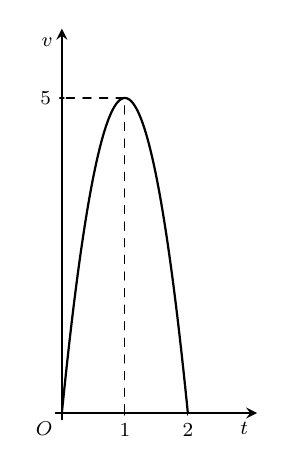
\begin{tikzpicture}[line join=round, line cap=round,>=stealth,font=\footnotesize,scale=0.8]
			\tikzset{every node/.style={scale=0.9}}
			\draw[->] (-0.1,0)--(3.1,0) node[below left] {$t$};
			\draw[->] (0,-0.1)--(0,6.1) node[below left] {$v$};
			\draw (0,0) node [below left] {$O$};
			\foreach \x/\nx in {1/1,2/2}
			\draw[thin] (\x,1pt)--(\x,-1pt) node [below] {$\nx$};
			\foreach \y/\ny in {5/5}
			\draw[thin] (1pt,\y)--(-1pt,\y) node [left] {$\ny$};
			\draw[dashed,thin](1,0)--(1,5)--(0,5);
			\begin{scope}
				\clip (0,0) rectangle (3,6);
				\draw[samples=200,domain=0:2,smooth,thick,variable=\x] plot (\x,{-5*(\x)^2+10*(\x)+0});
			\end{scope}
		\end{tikzpicture}
	\end{center}
	Gia tốc của vật tại thời điểm $t=1{,}5$ (s) bằng
	\shortans{$-5$}
	\loigiai{
		Giả sử đường parabol đi qua gốc tọa độ có dạng $y=at^2+bt$.\\
		Vì parabol đi qua các điểm $(2;0)$ và $(1;5)$ nên ta có hệ
		$$\heva{& 4a+2b=0 \\ & a+b=5}\Leftrightarrow \heva{& a=-5 \\ & b=10.}$$
		Vậy $v(t)=-5t^2+10t$, suy ra $a(t)=v'(t)=-10t+10$.\\
		Tại $t=1{,}5$ (s) thì $a\left(1{,}5\right)=-10\cdot 1{,}5+10=-5$ (m/s$^2$).
	}
\end{bt}

\begin{ex}%[1D7H3-3]
% nguon: Archive/2025-Sangtac/Khoi11/HK2/Data/1-CD/CD_1-OTHK2_De03.tex #4524

Chuyển động của một vật có phương trình $s(t)=4\cos\left(2\pi t-\dfrac{\pi}{12}\right)$ m, với $t$ là thời gian tính bằng giây. Khi đó
\choiceTF
{\True $s^{\prime}(t)=-8\pi\sin\left(2\pi t-\dfrac{\pi}{12}\right)$}
{$s^{\prime\prime}(t)=16\pi^2\cos\left(2\pi t-\dfrac{\pi}{12}\right)$}
{\True Vận tốc của vật tại thời điểm khi $t=5$ s là 
$s'(5)= 6{,}505\text{ m/s}$}
{Gia tốc của vật tại thời điểm khi $t=5$ s là $s''(5)\approx 152,533$ m/s$^2$}
\loigiai{
		\begin{itemchoice}
		\itemch  Đúng. Vì ta có $s^{\prime}(t)=-8\pi\sin\left(2\pi t-\dfrac{\pi}{12}\right)$.
		\itemch  Sai. Vì ta có $s^{\prime}(t)=-8\pi\sin\left(2\pi t-\dfrac{\pi}{12}\right)$ và $s^{\prime\prime}(t)=-16\pi^2\cos\left(2\pi t-\dfrac{\pi}{12}\right)$.
		\itemch  Đúng. Vì vận tốc tức thời của vật tại thời điểm $t=5$ s là \\
$s^{\prime}(5)=-8\pi\sin\left(10\pi-\dfrac{\pi}{12}\right)\approx 6{,}505$ (m/s).
	\itemch  Sai. Vì gia tốc tức thời của vật tại thời điểm $t=5$ s là\\
$s^{\prime\prime}(5)=-16\pi^2\cos\left(10\pi-\dfrac{\pi}{12}\right)\approx-152{,}533$ (m/s$^2$).
\end{itemchoice}
}
\end{ex}

\begin{ex}%[1D7H3-3]
% nguon: Archive/2025-Sangtac/Khoi11/HK2/Data/1-CD/CD_1-OTHK2_De02.tex #4528

	Chuyển động của một vật có phương trình $s(t)=4\cos \left(2\pi t-\dfrac{\pi}{6}\right)$\,(m), với $t$ là thời gian tính bằng giây, lấy $\pi^2=10$. Khi đó
	\choiceTF
	{\True $s'(t)=-8\pi \sin \left(2\pi t-\dfrac{\pi}{6} \right)$}
	{$s''(t)=16\pi^2\cos \left( 2\pi t-\dfrac{\pi}{6} \right)$}
	{\True Vận tốc của vật tại thời điểm khi $t=\dfrac{1}{2}$\,s là $-4\pi$\,(m/s)}
	{Gia tốc của vật tại thời điểm khi $t=\dfrac{1}{2}$\,s là $-80\sqrt 3$\,(m/s$^2$)}
	\loigiai{
		\begin{itemchoice}
		\itemch {\bf Đúng}.\\
		$s'(t)=-8\pi \sin \left(2\pi t-\dfrac{\pi}{6}\right)$.
		\itemch {\bf Sai}.\\
		$s''(t)=-16\pi^2\cos \left(2\pi t-\dfrac{\pi}{6}\right)$.
		\itemch {\bf Đúng}.\\
		Vận tốc của vật tại thời điểm khi $v=s'\left(\dfrac{1}{2}\right)=-4\pi$\,(m/s).
		\itemch {\bf Sai}.\\
		Gia tốc của vật tại thời điểm khi $t=\dfrac{1}{2}$\,s là $a=s''\left( \dfrac{1}{2}\right)=80\sqrt 3$\,(m/s$^2$).
		\end{itemchoice}
	}
\end{ex}

\begin{bt}%[1D7V2-8]
% nguon: Archive/2025-Sangtac/Khoi11/HK2/Data/1-CTST/CTST_1-OTGK2_De06.tex #4602

Vào một đêm yên tĩnh tại một ngọn núi nào đó ở Việt Nam. Giả sử các thông tin thu thập được từ các vệ tinh cho ta biết ngọn núi này được thể hiện bởi hàm số $y = f(x)= 100x - x^2$. Đột nhiên, từ trên trời xuất hiện một con quái vật ngoài hành tinh, được xem là mối nguy hiểm cho toàn thế giới. Tuy nhiên, con quái vật này có một điểm yếu là nếu ta bắn vào lõi năng lượng nằm tại giữa ngực của con quái vật, có toạ độ $(50; 3076)$ thì nó sẽ bị tiêu diệt. Khi đó các chiến sĩ từ quân đội nhân dân Việt Nam đã lên kế hoạch để bắn hạ con quái vật này bằng một chiếc xe tăng hạng nặng đang chuẩn bị xuất phát từ mặt đất. Giả sử quỹ đạo của đạn bắn sẽ là đường tiếp tuyến tại vị trí mà xe đứng trên ngọn núi. Các bạn hãy tưởng tượng mình là một trong những các nhà khoa học được quân đội nhân Việt Nam liên hệ để có thể tìm lời giải đáp cho vấn đề khẩn cấp này. Giả sử $(x_0, y_0)$ là toạ độ của vị trí xe tăng để có thể bắn hạ quái vật $(x_0 <50)$. Hãy tính $x_0 +y_0$.
\begin{center}
\tikzset{every picture/.style={line width=0.75pt}} %set default line width to 0.75pt        

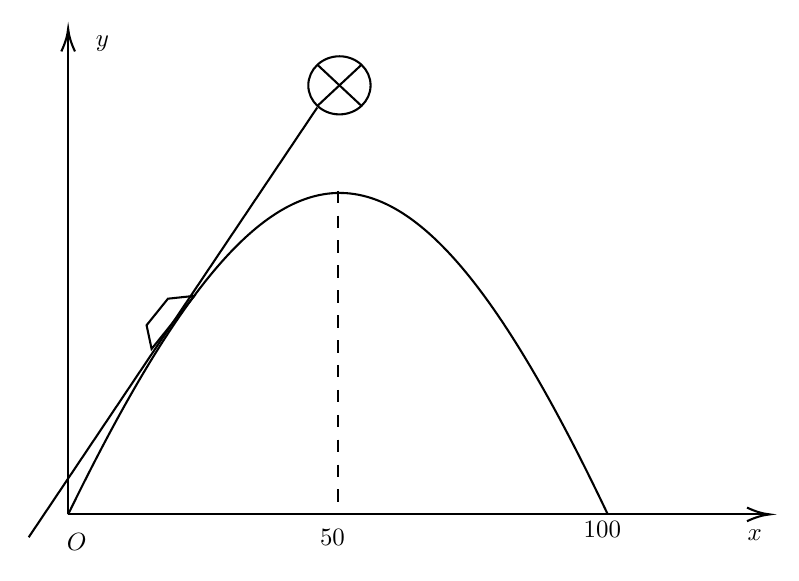
\begin{tikzpicture}[x=0.75pt,y=0.75pt,yscale=-1,xscale=1]
%uncomment if require: \path (0,300); %set diagram left start at 0, and has height of 300

%Straight Lines [id:da6221064196911785] 
\draw    (52,234) -- (52,2) ;
\draw [shift={(52,0)}, rotate = 90] [color={rgb, 255:red, 0; green, 0; blue, 0 }  ][line width=0.75]    (10.93,-3.29) .. controls (6.95,-1.4) and (3.31,-0.3) .. (0,0) .. controls (3.31,0.3) and (6.95,1.4) .. (10.93,3.29)   ;
%Straight Lines [id:da8745385467147941] 
\draw    (52,234) -- (388,234) ;
\draw [shift={(390,234)}, rotate = 180] [color={rgb, 255:red, 0; green, 0; blue, 0 }  ][line width=0.75]    (10.93,-3.29) .. controls (6.95,-1.4) and (3.31,-0.3) .. (0,0) .. controls (3.31,0.3) and (6.95,1.4) .. (10.93,3.29)   ;
%Curve Lines [id:da2599137458250198] 
\draw    (52,234) .. controls (152,29) and (213,26) .. (312,234) ;
%Shape: Diagonal Stripe [id:dp23363289838090973] 
\draw   (100.08,130.08) -- (112.79,128.72) -- (92.21,154.28) -- (89.79,142.86) -- cycle ;
%Flowchart: Summing Junction [id:dp7068757198064508] 
\draw   (167.71,27.28) .. controls (167.71,19.55) and (174.43,13.28) .. (182.71,13.28) .. controls (191,13.28) and (197.71,19.55) .. (197.71,27.28) .. controls (197.71,35.02) and (191,41.28) .. (182.71,41.28) .. controls (174.43,41.28) and (167.71,35.02) .. (167.71,27.28) -- cycle ; \draw   (172.11,17.38) -- (193.32,37.18) ; \draw   (193.32,17.38) -- (172.11,37.18) ;
%Straight Lines [id:da28229089728495715] 
\draw    (33,245) -- (172,38) ;
%Straight Lines [id:da004067916988188536] 
\draw  [dash pattern={on 4.5pt off 4.5pt}]  (182,78) -- (182,234) ;

% Text Node
\draw (378,240) node [anchor=north west][inner sep=0.75pt]   [align=left] {$\displaystyle x$};
% Text Node
\draw (64,2) node [anchor=north west][inner sep=0.75pt]   [align=left] {$\displaystyle y$};
% Text Node
\draw (50,242) node [anchor=north west][inner sep=0.75pt]   [align=left] {$\displaystyle O$};
% Text Node
\draw (172,240) node [anchor=north west][inner sep=0.75pt]   [align=left] {$\displaystyle 50$};
% Text Node
\draw (299,236) node [anchor=north west][inner sep=0.75pt]   [align=left] {$\displaystyle 100$};


\end{tikzpicture}

\end{center}
        \shortans[0]{1950}
	  \loigiai{Ta có $y = 100x - x^2$. Tọa độ quái vật là $(50,3076)$.
   Phương trình tiếp tuyến  tại $(x_0; y_0)$ có dạng $y = y_0 + y'(x_0)(x-x_0)$.\\
   Ta có $y'=100-2x$ nên phương trình tiếp tuyến có dạng $y = y_0 + (100 - 2x_0)(x-x_0)$.\\
   Phương trình này đi qua điểm $(50,3076)$ nên $3076 = y_0 + (100-2x_0)(50-x_0)$.\\
   Hơn nữa ta có $y_0 = 100x_0 -x_0^2$.\\
   Từ đó ta có $x_0^2-100x_0+1924 = 0 \Rightarrow x_0= 26 \text{ (vì $x_0<50$)} \Rightarrow y_0=1924$.\\
   Vậy $x_0 + y_0 = 1950$.
   
}
\end{bt}

\begin{bt}%[1D7V1-5]
% nguon: Archive/2025-Sangtac/Khoi11/HK2/Data/1-CTST/CTST_1-OTGK2_De01.tex #4622
%[Câu 19]
	Cho một vật chuyển động theo phương trình $s(t)=-t^2+40t+10$ trong đó $s$ là quãng đường vật đi được (đơn vị $m$), $t$ là thời gian chuyển động (đơn vị $s$). Tại thời điểm vật dừng lại thì vật đi được quãng đường bằng bao nhiêu mét?
	\shortans{$410$}
	\loigiai{
	\begin{align*}
		v(t) &=s'(t)\\
		&=-2t+40.
	\end{align*}
		Tại thời điểm vật dừng lại thì 
		\begin{align*}
			&~ v(t)=0\\ 
			\Leftrightarrow &~-2t+40=0\\ 
			\Leftrightarrow &~t=20.
		\end{align*}
		Quãng đường tại thời điểm vật dừng lại là
			\begin{align*}
			s(20) &=-20^2+40\cdot 20+10\\
			&=410.
		\end{align*}
	}
\end{bt}

\begin{bt}%[1D7V2-8]
% nguon: Archive/2025-Sangtac/Khoi11/HK2/Data/1-CTST/CTST_1-OTHK2-De02.tex #4627
%[Dự án soạn đề kiểm tra Toán 11 HKII NH24-25- Mui Doan]%[CTST_1_OTHK2-De02]
	Dân số của một thị trấn ven biển (tính bằng nghìn người) được mô hình hóa bởi hàm số $P(t)=\dfrac{300t^2}{t^2+4}$, trong đó $t$ là số năm kể từ năm $2020$. Tìm tốc độ tăng dân số năm $2028$. (Kết quả làm tròn đến hằng phần mười).
	
	\shortans{$-2{,}9$}
	\loigiai{
		Ta có $P'(t)=\dfrac{600t\left(t^2+4\right)-300t^2\cdot 2t}{\left(t^2+4\right)^2}=\dfrac{-2400t}{\left(t^2+4\right)^2}$.\\
		Từ năm $2020$ đến năm $2028$ có $2028-2020=8$ năm.\\
		Tốc độ tăng dân số tại thời điểm $t=8$ là
		$P'(8)=\dfrac{-2024\cdot 8 }{\left(8^2+4\right)^2}=-3{,}5$ (nghìn người/năm).
	}
\end{bt}

\begin{ex}%[1D7H3-3]
% nguon: Archive/2025-Sangtac/Khoi11/HK2/Data/1-CTST/CTST_1-OTHK2-De01.tex #4635
%[Dự án soạn đề kiểm tra Toán 11 HKII NH24-25- Thanh Phong]%[CTST_1_OTHK2-De01]
	Vị trí của một vật chuyển động thẳng được cho bởi phương trình \break $s(t)=\dfrac{1}{3} t^3-\dfrac{3}{2} t^2+3t$, trong đó $t$ được tính bằng giây và $s$ được tính bằng mét. 
	\choiceTF
	{\True Vận tốc tức thời của vật tại thời điểm $t=3$ bằng $3$ m/s}
	{Gia tốc tức thời của vật tại thời điểm $t=2$ bằng $1{,}5$ m/$s^2$}
	{\True Vận tốc của vật tăng dần trong khoảng thời gian từ giây thứ  $3$  đến giây thứ $5$}
	{Trong thời gian từ giây thứ  $1$  đến giây thứ $4$, vật có vận tốc nhỏ nhất bằng $1$ m/s}
	\loigiai{
		\begin{itemchoice}
			\itemch \textbf{Đúng}. Ta có $v(t)=s'(t)=t^2-3t+3$.\\
			 Vận tốc tức thời của vật tại thời điểm $t=3$ là 
			$v(3)=s'(3)=3^2-3 \cdot 3 +3=3$ m/s.
			\itemch \textbf{Sai}. Ta có $a(t)=v'(t)=2t-3$.\\
			Gia tốc tức thời của vật tại thời điểm $t=2$ là 
			$a(2)=v'(2)=2 \cdot 2-3=1$ m/s$^2$.
			\itemch \textbf{Đúng}.  Ta có $v(t)=\left(t-\dfrac{3}{2}\right)^2+\dfrac{3}{4}>0$.\\
			Bảng biến thiên
			\begin{center}
				
\begin{tikzpicture}
				\tkzTabInit[espcl=5,lgt=1.5,nocadre]
				{$t$/0.7,$v'(t)$/0.7,$v(t)$/2.1}
				{$3$,$5$}
				\tkzTabLine{,+,}
				\tkzTabVar{-/$3$,+/$13$}
				\end{tikzpicture}
			\end{center}
			Dựa vào bảng biến thiên, ta thấy vận tốc của vật tăng dần trong khoảng thời gian từ giây thứ  $3$  đến giây thứ $5$.
			\itemch \textbf{Sai}.  Ta có $a(t)=0\Leftrightarrow t= \dfrac{3}{2}$.\\
			Bảng biến thiên
			\begin{center}
				
\begin{tikzpicture}
				\tkzTabInit[espcl=2.5,lgt=1.5,nocadre]
				{$t$/1,$a'(t)$/0.7,$v(t)$/2.1}
				{$1$,$\dfrac{3}{2}$,$4$}
				\tkzTabLine{,-,0,+}
				\tkzTabVar{+/$1$,-/$\dfrac{3}{4}$,+/$7$}
				\end{tikzpicture}
			\end{center}
			Dựa vào bảng biến thiên, trong thời gian từ giây thứ  $1$  đến giây thứ $4$, vật có vận tốc nhỏ nhất bằng $\dfrac{3}{4}$ m/s.
		\end{itemchoice}
	}
\end{ex}

\begin{bt}%[1D7V2-8]
% nguon: Archive/2025-Sangtac/Khoi11/HK2/Data/1-CTST/CTST_1-OTHK2-De01.tex #4639
%[Dự án soạn đề kiểm tra Toán 11 HKII NH24-25- Thanh Phong]%[CTST_1_OTHK2-De01]
	Dân số $P$ (tính theo nghìn người) của một thành phố nhỏ được cho bởi công thức $P(t)=\dfrac{500t}{t^2+9}$, trong đó $t$ là thời gian được tính bằng năm. Tìm tốc độ tăng dân số tại thời điểm $t=12$. (Kết quả làm tròn đến hằng phần mười).
	
	\shortans{$-2{,}9$}
	\loigiai{
		Ta có $P'(t)=\dfrac{500\left(t^2+9\right)-500t\cdot 2t}{\left(t^2+9\right)^2}=\dfrac{-500t^2+4500}{\left(t^2+9\right)^2}$.\\
		Tốc độ tăng dân số tại thời điểm $t=12$ là
		$$P'(12)=\dfrac{-500\cdot 12^2+4500}{\left(12^2+9\right)^2}\approx -2{,}9\,\text{(nghìn người/năm)}.$$
	}
\end{bt}
